%% ============================================================
%% NOTE: This paper is formatted for Expert Systems with Applications
%% (Elsevier). To compile with the official template, change the
%% documentclass to:  \documentclass[preprint,12pt,authoryear]{elsarticle}
%% and replace the title/author block with elsarticle frontmatter.
%% The elsarticle.cls file can be obtained from:
%%   https://www.elsevier.com/researcher/author/policies-and-guidelines/latex-instructions
%% ============================================================
\documentclass[12pt,a4paper]{article}

%% Packages
\usepackage[margin=2.5cm]{geometry}
\usepackage{amsmath,amssymb,amsfonts}
\usepackage{algorithmic}
\usepackage{algorithm}
\usepackage{graphicx}
\usepackage{textcomp}
\usepackage{xcolor}
\usepackage{booktabs}
\usepackage{multirow}
\usepackage{pgfplots}
\pgfplotsset{compat=1.17}
\usepackage{tikz}
\usetikzlibrary{arrows.meta,positioning,calc}
\usepackage{subcaption}
\usepackage{hyperref}
\usepackage{url}
\usepackage{lineno}
\usepackage{natbib}
\usepackage{setspace}
\onehalfspacing

\modulolinenumbers[5]

%% Journal header
\newcommand{\journalname}{Expert Systems with Applications}

\begin{document}

\begin{center}
{\LARGE\bfseries Risk-Aware Corridor-Constrained Pathfinding for UAV Navigation in Biosecurity-Sensitive Environments\par}
\vspace{1em}
{\large Amr Elshahed$^{*}$, Majid Khan Bin Majahar Ali, Ahmad Sufril Azlan Mohamed, Farah Aini Binti Abdullah\par}
\vspace{0.5em}
{\itshape School of Computer Sciences, Universiti Sains Malaysia, 11800 Penang, Malaysia\par}
\vspace{0.3em}
{$^{*}$Corresponding author: \texttt{amr.elshahed@student.usm.my}\par}
\vspace{1.5em}
{\small Submitted to: \journalname\par}
\end{center}
\vspace{1em}

\begin{abstract}
Grid-based pathfinding underpins autonomous UAV navigation in biosecurity-sensitive environments, yet classical algorithms struggle with risk-weighted cost functions and dynamic obstacle changes that characterise real-world operations.
This paper investigates corridor-constrained pathfinding---via Incremental Line Search (ILS), its density-adaptive variant Adaptive ILS (AILS), and a new Risk-Responsive ILS (RILS)---on risk-annotated grids where traversal cost combines distance with spatial risk.
RILS adapts corridor width to the local risk distribution rather than obstacle density, achieving superior path quality ($\leq 0.1\%$ suboptimal on hotspot risk at $\lambda \leq 1.0$, versus $0.7$--$1.2\%$ for ILS/AILS) at the cost of lower speedup, providing a path-quality-oriented option for safety-critical applications.
Thirteen coordinated experiments evaluate the approach across risk-annotated grids (over 6,000 planned paths), procedurally generated port environments, Jump Point Search comparison, D*~Lite and Weighted A* baselines, corridor width sensitivity analysis, Moving AI Lab benchmarks (including risk-annotated and maze topologies), a multi-heuristic comparison, and progressive obstacle discovery missions.
Results demonstrate that ILS achieves up to $7.90\times$ speedup on risk-annotated grids with $86\%$ node reduction on gradient and uniform risk distributions, while maintaining path quality within $0.2\%$ for moderate risk weights ($\lambda \leq 1.0$).
On port environment grids, ILS achieves $1.0$--$3.9\times$ speedup scaling with grid size, reaching $75\%$ node reduction on $500 \times 500$ grids.
On uniform-cost grids, ILS surpasses Jump Point Search at obstacle densities $\geq 20\%$---a finding that reframes the relationship between corridor-based and symmetry-breaking methods.
Formal analysis establishes heuristic admissibility and sub-optimality bounds for corridor-restricted search on risk-weighted grids.
These findings establish corridor-constrained pathfinding as a practical acceleration layer for risk-aware autonomous navigation in biosecurity applications.
\end{abstract}

\noindent\textbf{Keywords:} Pathfinding; Grid search; Corridor constraint; Risk-aware planning; UAV navigation; Biosecurity; A* algorithm; Incremental Line Search; D* Lite; Weighted A*

\linenumbers

%% ====================================================================
\section{Introduction}\label{sec:intro}
%% ====================================================================

Autonomous unmanned aerial vehicles (UAVs) are increasingly deployed in biosecurity-sensitive operations, including contamination surveillance in port facilities, agricultural pest monitoring, and quarantine zone inspection~\citep{WHO2021,FAO2023}.
These missions impose two intertwined requirements on pathfinding algorithms: computational efficiency sufficient for real-time re-planning, and the ability to reason about spatially varying risk, because routes through high-risk zones (contamination gradients, quarantine boundaries, active inspection areas) may be operationally unacceptable even if they are distance-optimal.

Classical grid-based pathfinding algorithms---A*, Dijkstra, and their variants---produce optimal paths on standard occupancy grids but suffer from quadratic state-space growth as grid dimensions increase.
The problem intensifies on risk-annotated grids, where each cell carries both traversability and a continuous risk value, and the cost function becomes $\mathrm{cost} = \mathrm{dist} + \lambda \cdot \mathrm{risk}(cell)$ with a user-specified weight~$\lambda$.
The additional cost term reshapes the search landscape, forcing the planner to evaluate composite costs at every node expansion and often routing paths away from the geometric shortest path.

Several acceleration techniques address standard pathfinding.
Jump Point Search (JPS)~\citep{Harabor2011} eliminates symmetric path expansions on uniform-cost grids, achieving order-of-magnitude speedups.
Hierarchical methods such as HPA*~\citep{Botea2004} and Contraction Hierarchies~\citep{Geisberger2008} deliver fast queries after expensive preprocessing.
Incremental planners (D*~Lite~\citep{Koenig2002}, LPA*~\citep{Koenig2004}) reuse previous search trees when the map changes between queries.
However, none of these techniques simultaneously satisfies the requirements of biosecurity UAV navigation: JPS is structurally restricted to uniform-cost grids and cannot handle risk-weighted costs; hierarchical methods require stable maps that invalidate their preprocessing upon obstacle changes; and incremental planners incur high overhead when changes are large and clustered---the typical pattern when newly identified contamination zones or updated quarantine boundaries affect contiguous areas rather than isolated cells.

This paper investigates corridor-constrained pathfinding as an acceleration layer that addresses this gap.
The core idea, formalised as Incremental Line Search (ILS)~\citep{Elshahed2025ILS} and its density-adaptive variant Adaptive ILS (AILS)~\citep{Elshahed2025AILS}, restricts the search space to a spatial corridor centred on the Bresenham line between start and goal, expanding the corridor incrementally only when the initial search fails to find a path.
Prior work has demonstrated ILS and AILS on standard occupancy grids with substantial performance gains (87.31\% execution-time reduction for ILS, 76.8\% node reduction for AILS on $500 \times 500$ grids).
However, the application to risk-weighted grids---where the corridor's interaction with the risk landscape creates qualitatively different optimality--efficiency tradeoffs---has not been investigated.

\paragraph{Contributions.}
This paper makes six contributions:

\begin{enumerate}
\item A systematic evaluation of ILS on risk-annotated grids across three risk distributions, six risk-weight parameters, and three obstacle densities, demonstrating speedups of up to $7.90\times$ with $86\%$ node reduction while preserving path quality within $0.2\%$ for gradient and uniform risk at $\lambda \leq 1.0$.

\item An empirical demonstration that \emph{Risk-Responsive ILS} (RILS), a new variant adapting corridor width to local risk levels, achieves the best path quality among all corridor methods ($\leq 0.1\%$ suboptimal on hotspot risk vs.\ $0.7$--$1.2\%$ for ILS/AILS at $\lambda \leq 1.0$) but does \emph{not} improve speedup---an honest negative result that clarifies the tradeoff between risk-adaptive corridor construction and search-space restriction, positioning RILS as a path-quality-oriented option for safety-critical applications.

\item Formal sub-optimality analysis establishing heuristic admissibility, corridor containment properties, and empirically validated sub-optimality bounds for corridor-restricted search on risk-weighted grids.

\item Comprehensive baseline comparisons against D*~Lite~\citep{Koenig2002} and Weighted A*~\citep{Pohl1970}, demonstrating corridor-based methods' competitive advantages in different operational scenarios.

\item A domain-specific validation on procedurally generated container-port grids with structured obstacle layouts and biosecurity risk layers, revealing strong ILS performance scaling with grid size ($1.0$--$3.9\times$ speedup) alongside a grid-size threshold effect for AILS where adaptive-corridor overhead exceeds benefits on grids below $500 \times 500$.

\item A progressive obstacle discovery simulation across 180 sustained UAV missions revealing that corridor-constrained re-planning achieves higher mission success rates than standard A* (up to $73.3\%$ vs.\ $60.0\%$) with $12.6\%$ cumulative node reduction, at the cost of elevated path suboptimality.
\end{enumerate}

The remainder of this paper is organised as follows.
Section~\ref{sec:related} reviews related work on grid-based pathfinding, risk-aware planning, and search-space restriction techniques.
Section~\ref{sec:method} presents the ILS, AILS, and RILS algorithms adapted for risk-weighted grids, along with formal sub-optimality analysis.
Section~\ref{sec:experiments} describes the experimental design across thirteen coordinated experiments.
Section~\ref{sec:results} reports and analyses the results.
Section~\ref{sec:discussion} synthesises the findings and discusses implications for biosecurity UAV operations.
Section~\ref{sec:conclusion} concludes the paper.


%% ====================================================================
\section{Related Work}\label{sec:related}
%% ====================================================================

\subsection{Classical Grid-Based Pathfinding}

Grid-based pathfinding has been studied extensively in robotics and artificial intelligence.
Dijkstra's algorithm~\citep{Dijkstra1959} finds shortest paths on weighted graphs but explores the entire reachable space.
A*~\citep{Hart1968} reduces exploration through heuristic guidance, achieving optimality with admissible heuristics.
Bidirectional search variants reduce average-case complexity by searching from both endpoints~\citep{Goldberg2005}.
These algorithms form the baseline against which acceleration techniques are measured.

\subsection{Symmetry-Breaking and Jump Point Search}

Jump Point Search~\citep{Harabor2011} achieves dramatic speedups by identifying and pruning symmetric path expansions on uniform-cost grids.
JPS+ with preprocessing~\citep{Harabor2014} further accelerates queries through precomputed jump point maps.
Subgoal graphs~\citep{Uras2013} and rectangular symmetry reduction~\citep{Harabor2014RSR} offer alternative symmetry-exploitation strategies.
A fundamental limitation shared by all symmetry-based methods is their restriction to uniform-cost grids: the pruning rules that identify symmetric paths rely on the assumption that all traversable cells have identical cost, which breaks down on risk-annotated grids where cell costs vary spatially.

\subsection{Hierarchical and Preprocessing-Based Methods}

HPA*~\citep{Botea2004} decomposes the grid into clusters with precomputed inter-cluster paths, enabling fast query-time planning at the cost of offline preprocessing.
Contraction Hierarchies~\citep{Geisberger2008} contract the graph by adding shortcut edges, achieving near-constant query time on road networks.
Navigation meshes~\citep{Tozour2002} represent free space as convex polygons for efficient any-angle pathfinding, while Theta*~\citep{Nash2007} enables any-angle paths on grids through line-of-sight checks.
These methods require stable environments; dynamic obstacle changes invalidate the preprocessing and necessitate costly updates.

\subsection{Incremental and Dynamic Re-planning}

D*~Lite~\citep{Koenig2002} and LPA*~\citep{Koenig2004} maintain a search tree that can be repaired incrementally when the map changes between queries.
Field D*~\citep{Ferguson2005} extends this to continuous-cost interpolation on grids.
These planners are optimal for small, frequent perturbations (e.g., a robot discovering single blocked cells as it moves) but suffer when changes are large and clustered, because the priority queue maintenance propagates updates through much of the search space.

\subsection{Risk-Aware and Exposure-Sensitive Planning}

Risk-aware pathfinding incorporates non-distance costs into the planning objective.
Composite cost functions of the form $\mathrm{cost} = \mathrm{dist} + \lambda \cdot \mathrm{risk}$ have been applied in military route planning~\citep{Rowe1990}, hazardous materials transport~\citep{Erkut1998}, and UAV mission planning~\citep{Aggarwal2020}.
The challenge is that risk weighting reshapes the cost landscape, potentially routing optimal paths far from the geometric shortest path, which increases computational cost.
Alternative approaches include bounded-suboptimal methods that trade optimality for speed through heuristic inflation, as discussed in Section \ref{subsec:bounded}, or sampling-based and learning-based techniques reviewed in Sections \ref{subsec:sampling} and \ref{subsec:uav_learning}.
Corridor-based restriction offers a complementary approach: by confining search to a spatial band around the expected path direction, it limits the additional nodes that risk weighting forces into consideration.

\subsection{Bounded-Suboptimal Search}\label{subsec:bounded}

Bounded-suboptimal search methods trade optimality for computational speed by systematically relaxing the optimality requirement.
Weighted A* (wA*)~\citep{Pohl1970} multiplies the heuristic by a weight factor $w > 1$, yielding solutions guaranteed to be within a factor of $w$ of optimal (i.e., $w$-bounded suboptimal), typically with dramatic speedup: $f = g + w \cdot h$.
Anytime Weighted A*~\citep{Hansen2007} extends this by running a sequence of searches with decreasing weight values, returning progressively better solutions as time permits.
Potential Search~\citep{Stern2014}, already cited above for its foundational work on bounded-cost corridors, uses a potential function to estimate path cost and prunes nodes that provably cannot lead to solutions within a user-specified cost bound.
Focal Search~\citep{Pearl1982} maintains two open lists and prioritizes nodes in a ``focal'' set within a bounded distance of the best-known solution cost.
A key distinction from corridor-based methods is their underlying mechanism: bounded-suboptimal approaches trade optimality for speed through \emph{heuristic inflation} (manipulating the evaluation function), whereas corridor-based methods achieve the speed--quality tradeoff through \emph{spatial restriction} (limiting the search space itself).
This fundamental difference implies different applicability profiles: heuristic inflation may degrade solution quality in risk-sensitive environments where cost inflation is unacceptable, while spatial restriction maintains optimality within a constrained region.

\subsection{Sampling-Based and Multi-Objective Planning}\label{subsec:sampling}

Sampling-based methods sidestep explicit grid discretization by randomly sampling the configuration space and constructing roadmaps or trees.
RRT* (Rapidly-exploring Random Tree Star)~\citep{Karaman2011} probabilistically achieves asymptotic optimality by iteratively expanding a tree with cost-based rewiring, enabling handling of complex cost functions and continuous configuration spaces.
PRM* and its variants~\citep{Karaman2011} extend Probabilistic Roadmaps for multi-query planning with optimality guarantees.
However, these methods lack completeness guarantees on discrete grids and require significant computational resources for convergence to near-optimal solutions in high-dimensional spaces.
Multi-objective path planning methods extend classical pathfinding to scenarios with multiple competing objectives.
NAMOA* (Namoa* for multi-objective A*)~\citep{Mandow2010} computes the set of Pareto-optimal paths, enabling decision-makers to balance multiple criteria (e.g., distance vs.\ risk vs.\ time).
While powerful for complex decision problems, these methods incur additional computational overhead compared to single-objective methods.
A key observation is that sampling-based and multi-objective methods excel in unstructured or continuous environments with complex cost functions, but for the structured grid environments typical of UAV port operations, classical grid-based acceleration techniques such as symmetry exploitation and spatial restriction offer superior computational efficiency without sacrificing optimality guarantees.

\subsection{Recent UAV Path Planning and Learning-Based Approaches}\label{subsec:uav_learning}

Recent advances in autonomous systems have explored learning-based approaches for UAV path planning.
Deep reinforcement learning (DRL) methods train neural networks to map observations to actions, potentially discovering novel planning strategies~\citep{Wang2023}.
Hybrid approaches combining classical planning algorithms with machine learning (e.g., learning heuristics or using DRL for configuration selection) have shown promise in adapting to dynamic environments~\citep{Garau2022}.
However, learning-based methods introduce critical limitations for biosecurity-critical operations: they require substantial training data specific to the operational environment, lack formal optimality or safety guarantees, and cannot easily encode hard constraints (e.g., ``avoid pathogen release zones'').
Classical grid-based methods with acceleration techniques remain the preferred choice for safety-critical applications where solution quality, completeness, and verifiability are paramount.

\subsection{Corridor-Based Search Restriction}

The idea of restricting search to a spatial corridor has roots in bounded-cost search~\citep{Stern2014} and beam search~\citep{Bisiani1987}, where the search frontier is pruned to a fixed-size beam.
\citet{Elshahed2025ILS} formalised this as Incremental Line Search (ILS), which constructs a corridor along the Bresenham line between start and goal and expands it incrementally when the initial search fails.
\citet{Elshahed2025AILS} extended this to Adaptive ILS (AILS), which uses integral images (summed area tables) for $O(1)$ local density queries and constructs a variable-width corridor whose radius adapts to local obstacle density.
Both methods were evaluated on standard occupancy grids, demonstrating substantial performance gains.
The present work extends these methods to risk-weighted grids and validates them in biosecurity-specific environments.


%% ====================================================================
\section{Methodology}\label{sec:method}
%% ====================================================================

\subsection{Problem Formulation}

We consider pathfinding on a 2D grid graph $G = (V, E, w)$ where $V$ is the set of traversable cells, $E$ connects 8-adjacent free cells, and $w: E \to \mathbb{R}^+$ assigns edge weights.
Each cell $v \in V$ has an optional risk value $\rho(v) \in [0, 1]$.
The cost of traversing an edge $(u, v) \in E$ is:
\begin{equation}\label{eq:cost}
    w(u, v) = d(u, v) + \lambda \cdot \rho(v)
\end{equation}
where $d(u, v)$ is the Euclidean movement cost ($1.0$ for cardinal, $\sqrt{2}$ for diagonal moves) and $\lambda \geq 0$ is the risk-weight parameter.
At $\lambda = 0$ the problem reduces to standard shortest-path planning; increasing $\lambda$ progressively penalises high-risk cells.

The objective is to find a path $\pi^* = (v_0, v_1, \ldots, v_k)$ from start $s = v_0$ to goal $g = v_k$ that minimises:
\begin{equation}\label{eq:objective}
    C(\pi) = \sum_{i=0}^{k-1} w(v_i, v_{i+1})
\end{equation}

\subsection{Incremental Line Search (ILS)}

ILS~\citep{Elshahed2025ILS} constrains A* search to a spatial corridor $\mathcal{C}$ centred on the Bresenham line $\ell(s, g)$ between start and goal.
The corridor is constructed as:
\begin{equation}\label{eq:corridor}
    \mathcal{C}(r) = \{v \in V : \min_{p \in \ell(s,g)} \|v - p\|_\infty \leq r\}
\end{equation}
where $r$ is the corridor half-width.
A* search is then restricted to $\mathcal{C}$: only cells within the corridor are expanded.
If the search fails (no path exists within $\mathcal{C}$), the corridor width is increased by $\Delta r$ and the search is re-run.
This expansion continues for up to $K_{\max}$ attempts.

The initial corridor width is set as a fraction $\alpha_0$ of the grid diagonal: $r_0 = \alpha_0 \cdot \sqrt{H^2 + W^2}$, where $H$ and $W$ are the grid dimensions.
Empirically, $\alpha_0 = 0.05$ (5\% of diagonal) provides a good balance between corridor tightness and path feasibility.

\begin{algorithm}[htb]
\caption{ILS: Incremental Line Search on Risk-Weighted Grid}
\label{alg:ils}
\begin{algorithmic}[1]
\REQUIRE Grid $G$, start $s$, goal $g$, risk weight $\lambda$, initial width $r_0$, max attempts $K_{\max}$
\ENSURE Path $\pi^*$ or FAILURE
\STATE $r \leftarrow r_0$
\FOR{$k = 1$ \TO $K_{\max}$}
    \STATE Build corridor $\mathcal{C}(r)$ via Bresenham line $\ell(s, g)$
    \STATE $\pi \leftarrow$ A*$(G|_{\mathcal{C}(r)}, s, g, \lambda)$ \COMMENT{Search restricted to $\mathcal{C}$}
    \IF{$\pi \neq$ NULL}
        \RETURN $\pi$
    \ENDIF
    \STATE $r \leftarrow r + \Delta r$ \COMMENT{Expand corridor}
\ENDFOR
\RETURN FAILURE
\end{algorithmic}
\end{algorithm}

\subsection{Adaptive ILS (AILS)}

AILS~\citep{Elshahed2025AILS} replaces the uniform-width corridor with a variable-width corridor whose radius at each reference-line cell adapts to local obstacle density.
The key mechanism is the integral image (summed area table) $I$, which enables $O(1)$ density queries:
\begin{equation}\label{eq:density}
    \delta(p, \omega) = \frac{1}{(2\omega+1)^2} \sum_{(r,c) \in W(p,\omega)} \mathbf{1}[\text{obstacle at } (r,c)]
\end{equation}
where $W(p, \omega)$ is the $(2\omega+1) \times (2\omega+1)$ window centred at point $p$ on the reference line.

The corridor radius at each reference point is:
\begin{equation}\label{eq:adaptive_radius}
    r(p) = r_{\min} + (r_{\max} - r_{\min}) \cdot \delta(p, \omega)^\alpha
\end{equation}
where $r_{\min}$ and $r_{\max}$ bound the corridor width, and $\alpha$ controls sensitivity to density changes.
High local density produces a wider corridor (to accommodate detours around obstacles); low density produces a narrow corridor (to maximise search-space exclusion).

\begin{algorithm}[htb]
\caption{AILS: Adaptive Incremental Line Search}
\label{alg:ails}
\begin{algorithmic}[1]
\REQUIRE Grid $G$, start $s$, goal $g$, risk weight $\lambda$, density exponent $\alpha$, window $\omega$, max attempts $K_{\max}$
\ENSURE Path $\pi^*$ or FAILURE
\STATE Build integral image $I$ over obstacle grid
\STATE Compute Bresenham line $\ell(s, g)$
\FOR{$k = 1$ \TO $K_{\max}$}
    \FOR{each point $p$ on $\ell(s, g)$}
        \STATE $\delta(p) \leftarrow$ density query via $I$ in window $W(p, \omega)$ \COMMENT{$O(1)$}
        \STATE $r(p) \leftarrow r_{\min} + (r_{\max} - r_{\min}) \cdot \delta(p)^\alpha$
    \ENDFOR
    \STATE $\mathcal{C} \leftarrow$ variable-width corridor with radius $r(p)$ at each $p$
    \STATE $\pi \leftarrow$ A*$(G|_{\mathcal{C}}, s, g, \lambda)$
    \IF{$\pi \neq$ NULL}
        \RETURN $\pi$
    \ENDIF
    \STATE $r_{\min} \leftarrow r_{\min} + \Delta r$; $r_{\max} \leftarrow r_{\max} + \Delta r$
\ENDFOR
\RETURN FAILURE
\end{algorithmic}
\end{algorithm}

\subsection{Risk-Aware Heuristic Adaptation}

On risk-weighted grids, the standard octile distance heuristic $h(n, g)$ remains admissible for $\lambda = 0$ but underestimates true cost when $\lambda > 0$ because it ignores risk contributions.
We adjust the heuristic as:
\begin{equation}\label{eq:heuristic}
    h_\lambda(n, g) = h(n, g) \cdot (1 + \lambda \cdot \bar{\rho})
\end{equation}
where $\bar{\rho}$ is a conservative estimate of mean risk along the remaining path (we use $\bar{\rho} = 0.3$ based on empirical grid statistics).
This adjustment maintains admissibility for moderate $\lambda$ values while improving search guidance.

\subsection{Risk-Responsive ILS (RILS)}\label{subsec:rils}

While AILS adapts corridor width based on local \emph{obstacle density}, its corridor may be inappropriately narrow in regions with sparse obstacles but elevated risk---precisely the areas where wider corridors are needed to allow risk-avoidance detours.
We propose Risk-Responsive ILS (RILS), a new variant that adapts corridor width to the local \emph{risk distribution} rather than obstacle density.

RILS constructs the corridor along the same Bresenham reference line as ILS and AILS, but determines the radius at each reference point $p$ using the local mean risk within a query window:
\begin{equation}\label{eq:risk_query}
    \bar{\rho}(p, \omega) = \frac{1}{(2\omega+1)^2} \sum_{(r,c) \in W(p,\omega)} \rho(r,c)
\end{equation}
where $W(p, \omega)$ is the $(2\omega+1) \times (2\omega+1)$ window centred at $p$ and $\rho(r,c)$ is the risk value at cell $(r,c)$.
This query is computed in $O(1)$ time using an integral image (summed area table) over the risk layer, analogous to AILS's density queries but operating on the continuous risk values rather than binary obstacle indicators.

The corridor radius at each reference point is:
\begin{equation}\label{eq:rils_radius}
    r_{\text{RILS}}(p) = r_{\text{base}} + (r_{\max} - r_{\text{base}}) \cdot \bar{\rho}(p, \omega)^\beta
\end{equation}
where $r_{\text{base}}$ is the minimum corridor width, $r_{\max}$ is the maximum width, and $\beta \geq 0$ controls risk-sensitivity.
In high-risk regions ($\bar{\rho} \to 1$), the corridor approaches $r_{\max}$, providing ample space for the search to find risk-avoidance detours.
In low-risk regions ($\bar{\rho} \to 0$), the corridor narrows toward $r_{\text{base}}$, maximising search-space pruning where risk avoidance is unnecessary.
When no risk layer is present ($\lambda = 0$), RILS degenerates to standard ILS.

The key distinction between AILS and RILS is their adaptation signal:
\begin{itemize}
    \item \textbf{AILS:} $r(p) \propto \delta(p)^\alpha$ where $\delta$ is local \emph{obstacle density}---wider corridors near obstacles to enable detours around blocked cells.
    \item \textbf{RILS:} $r(p) \propto \bar{\rho}(p)^\beta$ where $\bar{\rho}$ is local \emph{mean risk}---wider corridors in high-risk regions to enable risk-avoidance routing.
\end{itemize}

This distinction means RILS is specifically designed for risk-weighted grids where the cost landscape (not the obstacle layout) determines path optimality.
An open, obstacle-free region with high risk requires a wide corridor for RILS (to find risk-avoiding paths) but a narrow corridor for AILS (since obstacle density is zero)---precisely the scenario where AILS's adaptation signal is misleading.

Default parameters used in experiments: $r_{\text{base}} = 0.05 \cdot \text{diag}$, $r_{\max} = 0.15 \cdot \text{diag}$, $\beta = 1.0$, $\omega = 5$, up to 10 expansion attempts.

\begin{algorithm}[htb]
\caption{RILS: Risk-Responsive Incremental Line Search}
\label{alg:rils}
\begin{algorithmic}[1]
\REQUIRE Grid $G$, start $s$, goal $g$, risk weight $\lambda$, risk exponent $\beta$, window $\omega$, max attempts $K_{\max}$
\ENSURE Path $\pi^*$ or FAILURE
\STATE Build integral image $I_\rho$ over risk layer $\rho$
\STATE Compute Bresenham line $\ell(s, g)$
\FOR{$k = 1$ \TO $K_{\max}$}
    \FOR{each point $p$ on $\ell(s, g)$}
        \STATE $\bar{\rho}(p) \leftarrow$ mean risk query via $I_\rho$ in window $W(p, \omega)$ \COMMENT{$O(1)$}
        \STATE $r(p) \leftarrow r_{\text{base}} + (r_{\max} - r_{\text{base}}) \cdot \bar{\rho}(p)^\beta$
    \ENDFOR
    \STATE $\mathcal{C} \leftarrow$ variable-width corridor with radius $r(p)$ at each $p$
    \STATE $\pi \leftarrow$ A*$(G|_{\mathcal{C}}, s, g, \lambda)$
    \IF{$\pi \neq$ NULL}
        \RETURN $\pi$
    \ENDIF
    \STATE $r_{\text{base}} \leftarrow r_{\text{base}} + \Delta r$; $r_{\max} \leftarrow r_{\max} + \Delta r$
\ENDFOR
\RETURN FAILURE
\end{algorithmic}
\end{algorithm}

\begin{figure}[htb]
\centering

\includegraphics[width=\textwidth]{figures/corridor_comparison_real.pdf}
\caption{Corridor comparison on a $200 \times 200$ risk-annotated grid with hotspot risk ($\lambda = 1.0$, 20\% obstacle density). (a)~Grid with risk overlay (darker = higher risk) and A* optimal path. (b)~ILS uniform-width corridor (blue shading) with ILS path. (c)~AILS density-adaptive corridor (green shading). (d)~RILS risk-responsive corridor (red shading), which widens near high-risk hotspots to enable risk-avoidance routing. Grey cells are obstacles; green circle = start; red star = goal.}
\label{fig:corridor_comparison}
\end{figure}

\subsection{Formal Sub-Optimality Analysis}\label{subsec:formal}

We now establish theoretical properties of corridor-constrained search on risk-weighted grids.

\paragraph{Unconditionally admissible heuristic.}
The simplest admissible heuristic for risk-weighted grids uses $\bar{\rho} = 0$, reducing to the standard octile distance:
\begin{equation}\label{eq:h0}
    h_0(n, g) = h(n, g)
\end{equation}
Since $h(n,g) \leq d_{\min}(n,g) \leq C(\pi)$ for any path $\pi$, this heuristic is admissible for all $\lambda \geq 0$ and all risk distributions, unconditionally.
However, $h_0$ ignores risk and provides weak guidance when $\lambda > 0$.

\paragraph{Risk-adjusted heuristic (conditional).}
To improve search guidance, we use the risk-adjusted heuristic from Eq.~\ref{eq:heuristic}, restated here with explicit conditions:

\begin{proposition}[Conditional Heuristic Admissibility]\label{prop:admissible}
Let $h_\lambda(n, g) = h(n, g) \cdot (1 + \lambda \cdot \bar{\rho})$ with parameter $\bar{\rho} \geq 0$.
Then $h_\lambda$ is admissible for any node $n$ provided the following condition holds: the mean risk along every optimal path from $n$ to $g$ satisfies $\bar{\rho}_{\pi^*} \geq \bar{\rho}$.
\end{proposition}

\noindent\textit{Proof.}
For any path $\pi = (n, v_1, \ldots, g)$ with $k$ edges, the true cost is:
\[
C(\pi) = \sum_{i=0}^{k-1} [d(v_i, v_{i+1}) + \lambda \cdot \rho(v_{i+1})] = D(\pi) + \lambda \cdot R(\pi)
\]
where $D(\pi) \geq h(n,g)$ is the total distance cost and $R(\pi) = \sum_{i=1}^{k} \rho(v_i)$ is the cumulative risk.
Since the path traverses $k$ cells and $\bar{\rho}_\pi = R(\pi)/k$, we have $R(\pi) = k \cdot \bar{\rho}_\pi$.
For paths with at least as many steps as the octile distance, $k \geq h(n,g)$ (each step covers at most distance $\sqrt{2}$, but $h$ is the octile distance, so $k \geq \lceil h / \sqrt{2} \rceil$; more precisely, $D(\pi) \geq h(n,g)$ and since cardinal steps cost 1.0, $k \geq h(n,g)$ in the worst case).
When $\bar{\rho}_\pi \geq \bar{\rho}$:
\[
C(\pi) = D(\pi) + \lambda \cdot k \cdot \bar{\rho}_\pi \geq h(n,g) + \lambda \cdot h(n,g) \cdot \bar{\rho} = h_\lambda(n,g)
\]
Thus $h_\lambda(n,g) \leq C(\pi)$ for all paths satisfying the mean-risk condition.
$\square$

\paragraph{Practical implications.}
With $\bar{\rho} = 0.3$, the condition $\bar{\rho}_{\pi^*} \geq 0.3$ is satisfied for gradient risk (mean $\approx 0.5$), uniform risk (constant at $0.3$), and most hotspot configurations where the path traverses at least one high-risk zone.
In the rare case where the condition is violated (e.g., a short path through a zero-risk corridor), the heuristic may slightly overestimate, causing A* to behave as a greedy best-first search locally---still finding valid paths but potentially losing optimality guarantees.
Empirically, path quality remained within $0.2\%$ of optimal across all 5,400 tested configurations (Experiment~1), confirming that the condition holds in practice for the tested grid configurations.
For applications requiring guaranteed admissibility regardless of risk distribution, setting $\bar{\rho} = 0$ (the unconditionally admissible variant) is recommended, at the cost of weaker search guidance and potentially more node expansions.

\begin{proposition}[Corridor Containment and Completeness]\label{prop:complete}
If the optimal path $\pi^*$ lies entirely within corridor $\mathcal{C}(r)$, i.e., $\pi^* \subseteq \mathcal{C}(r)$, then corridor-restricted A* returns $\pi^*$.
Furthermore, the incremental expansion mechanism (up to $K_{\max}$ attempts) guarantees that if a path exists within a corridor of width $r_0 + K_{\max} \cdot \Delta r$, it will be found.
\end{proposition}

\noindent\textit{Proof.}
When $\pi^* \subseteq \mathcal{C}(r)$, the corridor restriction removes only nodes not on $\pi^*$, and A* with an admissible heuristic on the restricted graph $G|_{\mathcal{C}(r)}$ finds $\pi^*$ because all nodes on $\pi^*$ remain in the search space.
For completeness, each failed attempt increases corridor width by $\Delta r$, so after $K_{\max}$ attempts the corridor covers all cells within $\ell_\infty$-distance $r_0 + K_{\max} \cdot \Delta r$ of the reference line.
$\square$

\begin{corollary}[Sub-Optimality Bound]\label{cor:bound}
For a given corridor width $r$ and risk distribution, let $\pi_r^*$ be the optimal path within $\mathcal{C}(r)$ and $\pi^*$ be the globally optimal path.
Then $C(\pi_r^*) / C(\pi^*) \leq 1 + \Delta_r$, where $\Delta_r$ is the maximum additional cost incurred by the corridor constraint, bounded by $\Delta_r \leq 2 \cdot r \cdot \lambda \cdot \rho_{\max}$ for corridors of width $r$ on grids with maximum risk $\rho_{\max}$.
Empirically, $\Delta_r < 0.002$ for gradient and uniform risk at $\lambda \leq 1.0$ (Table~\ref{tab:exp1_speedup}), and $\Delta_r < 0.013$ for hotspot risk at $\lambda \leq 1.0$.
\end{corollary}

These bounds establish that corridor-constrained search is near-optimal when the corridor captures the globally optimal path or a close substitute.
The incremental expansion mechanism serves as a safety net: if the initial corridor is too narrow, successive expansions widen it until a feasible path is found.
The empirical path quality results in Sections~\ref{sec:results} confirm that these theoretical bounds are loose upper limits; actual sub-optimality is substantially smaller.

\paragraph{On tighter bounds.}
The bound $\Delta_r \leq 2 \cdot r \cdot \lambda \cdot \rho_{\max}$ is distribution-agnostic and therefore necessarily loose.
Distribution-specific tighter bounds may be achievable: for gradient risk (where $\rho$ varies smoothly), the maximum deviation from the corridor-restricted path to the globally optimal path is bounded by the local risk gradient magnitude, yielding $\Delta_r^{\text{grad}} \leq r \cdot \lambda \cdot \|\nabla \rho\|_{\max}$.
For uniform risk ($\rho = c$), $\Delta_r = 0$ trivially since all paths incur identical risk per unit distance.
Hotspot risk admits no simple tighter bound because the deviation depends on whether the optimal path's detour around a hotspot falls inside or outside the corridor---a configuration-dependent property.
Deriving tight $(1+\epsilon)$ bounds conditioned on specific risk distributions remains an open theoretical question.


%% ====================================================================
\section{Experimental Design}\label{sec:experiments}
%% ====================================================================

Thirteen coordinated experiments evaluate corridor-constrained pathfinding on risk-weighted grids.
Experiments~1--5 form the core evaluation; Experiments~6--9 address additional baselines, sensitivity analysis, and the RILS algorithm; Experiments~10--10c validate results on standard Moving AI Lab benchmarks (including risk-annotated and maze topologies); Experiment~11 evaluates heuristic sensitivity.
All experiments use 8-connected grid movement with octile distance heuristic (adjusted per Eq.~\ref{eq:heuristic} when $\lambda > 0$).
All reported confidence intervals are 95\% CIs computed from paired samples.
Experiments were conducted on an Intel Core i7-based system with 16~GB RAM.

\subsection{Experiment 1: Risk-Annotated Grids}

\paragraph{Setup.}
We generated $200 \times 200$ binary occupancy grids at three obstacle densities (10\%, 20\%, 30\%), each overlaid with one of three risk distributions: (i)~\emph{gradient} (risk increasing linearly from top-left to bottom-right), (ii)~\emph{hotspot} (Gaussian-centred high-risk zones), and (iii)~\emph{uniform} (constant risk across all cells).
Six risk-weight values were tested: $\lambda \in \{0, 0.1, 0.5, 1.0, 2.0, 5.0\}$.
For each density--risk--$\lambda$ configuration, 100 random maps were generated, for a total of 5,400 planned paths.
Start was fixed at $(0,0)$ and goal at $(199, 199)$.

\paragraph{Algorithms.}
Standard A* (baseline) and ILS~A* (5\% initial corridor width, up to 10 expansion attempts) were compared.
Metrics: runtime (ms), nodes expanded, path cost ratio (ILS/A*), cumulative risk exposure ratio, and corridor expansion count.

\paragraph{Statistical protocol.}
Paired $t$-tests and Cohen's $d$ effect sizes were computed for node-count differences at each configuration.
Significance threshold: $p < 0.05$.

\subsection{Experiment 2: Port Environment Validation}

\paragraph{Setup.}
Procedurally generated container-port grids reproduced the structural features of real port facilities: a quay zone (sparse, open), a container yard (rectangular blocks separated by narrow aisles), a gate zone (barriers with controlled openings), and a buffer zone (mixed clutter).
Biosecurity risk layers were overlaid, with elevated risk near container blocks (inspection zones) and gate checkpoints.
Three grid sizes ($200 \times 200$, $300 \times 300$, $500 \times 500$) and three risk weights ($\lambda \in \{0, 0.5, 1.0\}$) were tested.
Thirty start--goal pairs were evaluated per configuration (270 total).

\paragraph{Port generation parameters.}
The procedural port generator uses the following zone proportions relative to grid height: quay zone $0$--$15\%$, buffer $15$--$20\%$, container yard $20$--$70\%$, gate zone $75$--$85\%$, open area $85$--$100\%$.
Container blocks in the yard zone are $8$--$15$ cells wide and $3$--$6$ cells tall, separated by aisles of $2$--$3$ cells.
Gate barriers span the full grid width with $3$--$5$ controlled openings per barrier, each $3$--$5$ cells wide.
Risk values are assigned as: $0.7$--$0.9$ adjacent to container blocks (inspection zones), $0.5$--$0.7$ at gate checkpoints, $0.1$--$0.3$ in open/quay areas.

\paragraph{Algorithms.}
Standard A*, ILS~A*, and AILS~A* ($r_{\min} = 2$, $r_{\max} = \lceil 0.1 \cdot \min(H, W) \rceil$, $\alpha = 1.0$, $\omega = 3$).

\subsection{Experiment 3: JPS Comparative Evaluation}

\paragraph{Setup.}
To quantify how corridor-based methods compare with symmetry-breaking techniques on uniform-cost grids, we evaluated A*, ILS~A* (3\% corridor), and JPS on $200 \times 200$ grids at three densities (10\%, 20\%, 30\%) with 100 maps per density.
No risk layer was applied ($\lambda = 0$).
All algorithms, including JPS, were implemented from scratch in Python following the canonical descriptions in \citet{Harabor2011} for JPS and \citet{Hart1968} for A*.
Custom implementations were used rather than established libraries to ensure a fair comparison under identical language overhead and data structures.

\paragraph{Rationale.}
JPS cannot operate on risk-weighted grids; this experiment establishes the baseline comparison on JPS's home territory before demonstrating ILS's advantage on the risk-weighted grids where JPS is inapplicable.

\subsection{Experiment 4: Dynamic Re-planning}

\paragraph{Setup.}
To simulate re-planning after obstacle discovery, we computed an initial path on each grid, then inserted 5 obstacle clusters (radius 3 cells) along the path at approximately 40\% of its length.
Re-planning was initiated from the agent's pre-insertion position.
We compared A* full re-run and AILS corridor-constrained re-plan on $200 \times 200$ grids at three densities with 128 maps per density.

\subsection{Experiment 5: Progressive Obstacle Discovery}

\paragraph{Setup.}
Each simulated mission placed an agent at $(0,0)$ on a $200 \times 200$ grid with goal $(199, 199)$.
Every 20 steps, the agent's sensor (range 15 cells) discovered 3 new contamination points, each blocking a $3 \times 3$ cell cluster.
If the path ahead was blocked, the agent re-planned from its current position.
Sixty missions per density level (10\%, 20\%, 30\%) were simulated, producing approximately 12 re-plan events per mission.
Both A* and ILS~A* were evaluated.

\subsection{Experiment 6: Weighted A* Comparison}

\paragraph{Setup.}
To compare corridor-based restriction with heuristic-inflation-based acceleration, we evaluated Weighted A* (wA*) with weights $w \in \{1.5, 2.0, 3.0\}$ against A*, ILS, and AILS on $200 \times 200$ risk-annotated grids.
The same density--risk--$\lambda$ configurations as Experiment~1 were used, with 50 random maps per configuration.
Start and goal were placed at random positions (minimum Manhattan distance 100 cells) to diversify the path topology.

\paragraph{Rationale.}
wA* provides $w$-bounded suboptimal solutions~\citep{Pohl1970} and represents the standard bounded-suboptimal baseline.
This experiment directly compares two orthogonal acceleration strategies: heuristic inflation (wA*) versus spatial restriction (ILS/AILS).

\subsection{Experiment 7: Corridor Width Sensitivity}

\paragraph{Setup.}
To characterise the sensitivity of ILS performance to corridor width, we swept the initial corridor fraction $\alpha$ across values $\{0.01, 0.03, 0.05, 0.07, 0.10, 0.15, 0.20, 0.30\}$ on $200 \times 200$ risk-annotated grids at three densities and three risk distributions.
Fifty maps per configuration were evaluated with $\lambda = 1.0$, for a total of 3,600 planned paths.

\paragraph{Rationale.}
Prior experiments used a fixed $\alpha_0 = 0.05$.
This sweep identifies the optimal corridor width and characterises the speedup--quality Pareto frontier, providing practitioners with explicit guidance for parameter selection.

\subsection{Experiment 8: RILS Evaluation}

\paragraph{Setup.}
RILS (Section~\ref{subsec:rils}) was compared against A*, ILS, and AILS on $200 \times 200$ risk-annotated grids at three densities, three risk distributions, and three risk weights ($\lambda \in \{0.5, 1.0, 2.0\}$).
Fifty maps per configuration with random start--goal pairs (minimum distance 100 cells).
RILS parameters: $r_{\text{base}} = 0.05 \cdot \text{diag}$, $r_{\max} = 0.15 \cdot \text{diag}$, $\beta = 1.0$, $\omega = 5$.

\paragraph{Rationale.}
This experiment evaluates RILS's ability to exploit risk-distribution information for improved corridor construction, particularly on hotspot risk where standard ILS shows weaker performance.

\subsection{Experiment 9: Large-Grid AILS Validation}

\paragraph{Setup.}
To resolve the AILS grid-size threshold effect observed in Experiment~2, we evaluated AILS on $500 \times 500$ risk-annotated grids at three densities and three risk weights ($\lambda \in \{0.5, 1.0, 2.0\}$).
Thirty maps per configuration.

\paragraph{Rationale.}
Experiments~2 and 4 showed AILS incurring negative performance on grids $\leq 300 \times 300$.
This experiment validates AILS on grids above the hypothesised threshold, establishing its applicability range with statistical confidence.

\subsection{Experiment 10: Moving AI Lab Benchmark Evaluation}

\paragraph{Setup.}
To establish external validity and enable comparison with published results, we evaluated A*, ILS, and AILS on standard benchmark maps from the Moving AI Lab~\citep{Sturtevant2012}.
Three map categories were tested: (i)~\emph{game maps} from Dragon Age: Origins (4 maps: lak303d, den501d, brc202d, ost003d), featuring structured indoor environments with rooms and corridors; (ii)~\emph{mazes} (4 maps: maze512-$k$-0, $k \in \{1, 2, 4, 8\}$) with progressively wider corridors; and (iii)~\emph{random maps} (4 maps: random512-$d$-0, $d \in \{10, 20, 30, 40\}$\% density) matching the procedural grids used in Experiments~1--9.
All maps are $512 \times 512$ or smaller.
Up to 100 scenarios per map were selected from the official scenario files, preferring longer paths for a more meaningful evaluation.
No risk layer was applied ($\lambda = 0$); this experiment tests the corridor mechanism itself on diverse standard-benchmark topologies.
ILS used the default $\alpha = 0.05$; AILS used $r_{\min} = 0.02 \cdot \text{diag}$, $r_{\max} = 0.10 \cdot \text{diag}$.

\paragraph{Rationale.}
Experiments~1--9 used procedurally generated grids.
This experiment addresses the external validity concern by testing on established benchmarks with known optimal path lengths, enabling direct comparison with published methods and verifying that corridor-based acceleration generalises beyond the specific grid generation procedure used in prior experiments.

\subsection{Experiment 10b: Risk-Annotated Benchmark Evaluation}

\paragraph{Setup.}
To address the limitation of testing benchmarks only at $\lambda = 0$, we overlaid synthetic risk layers (gradient and hotspot distributions) on Moving AI Lab random maps and evaluated ILS, AILS, and RILS at $\lambda \in \{0.5, 1.0\}$.
Two random maps (random512-20-0, random512-30-0) were tested with 10 scenarios per configuration, selecting longer paths for meaningful evaluation.

\paragraph{Rationale.}
Experiment~10 demonstrated that corridor methods provide no benefit at $\lambda = 0$ on standard benchmarks.
This experiment tests whether adding risk layers to \emph{standardised} map topologies activates the corridor advantage, isolating the contribution of the risk-weighted cost landscape from the map generation procedure.

\subsection{Experiment 10c: Maze Benchmark Evaluation}

\paragraph{Setup.}
To stress-test corridor methods on adversarial topologies, we evaluated ILS and AILS on procedurally generated maze maps of size $256 \times 256$ with four corridor widths ($k \in \{1, 2, 4, 8\}$), corresponding to obstacle densities of 78\%, 52\%, 33\%, and 18\%.
Twenty scenarios per maze configuration were tested with no risk layer ($\lambda = 0$).
Mazes were generated using randomised DFS, producing perfect mazes where every cell is reachable.
Official Moving AI Lab maze maps could not be used due to persistent server-side download errors (HTTP 500) at the time of experiments; multiple download attempts across different dates returned error pages rather than map data.

\paragraph{Rationale.}
Maze topologies represent a worst case for corridor methods: paths require long detours through narrow passages that may lie far from the Bresenham reference line.
This experiment quantifies the performance degradation on adversarial topologies and establishes the boundary conditions for corridor applicability.

\subsection{Experiment 11: Multi-Heuristic Comparison}

\paragraph{Setup.}
To evaluate robustness to heuristic choice, we compared four heuristics within ILS at $\lambda = 1.0$: (i)~octile distance, (ii)~Euclidean distance, (iii)~Manhattan distance, and (iv)~risk-adjusted octile ($h_\lambda = h \cdot (1 + \lambda \cdot 0.3)$).
Each heuristic was tested with both standard A* and ILS ($\alpha = 0.05$) on $200 \times 200$ risk-annotated grids at three densities and three risk distributions (20 maps per configuration).

\paragraph{Rationale.}
All prior experiments used octile distance exclusively.
This experiment verifies that corridor-based speedups are robust across heuristic functions and identifies whether tighter (risk-adjusted) or weaker (Manhattan) heuristics interact differently with the corridor mechanism.


%% ====================================================================
\section{Results}\label{sec:results}
%% ====================================================================

\subsection{Experiment 1: Risk-Annotated Grids}

\subsubsection{Runtime Speedup}

Table~\ref{tab:exp1_speedup} presents ILS speedup over standard A* at $\lambda = 1.0$ across all nine density--risk combinations.

\begin{table}[htb]
\centering
\caption{Runtime speedup (ILS A*/Standard A*) at $\lambda = 1.0$ on $200 \times 200$ risk-annotated grids.}
\label{tab:exp1_speedup}
\begin{tabular}{lccc|c}
\toprule
\textbf{Density} & \textbf{Gradient} & \textbf{Hotspot} & \textbf{Uniform} & \textbf{Mean} \\
\midrule
10\% & $6.27\times$ & $1.73\times$ & $3.11\times$ & $3.70\times$ \\
20\% & $6.45\times$ & $1.70\times$ & $3.51\times$ & $3.89\times$ \\
30\% & $6.68\times$ & $1.80\times$ & $4.04\times$ & $4.17\times$ \\
\midrule
Mean & $6.47\times$ & $1.74\times$ & $3.55\times$ & $3.92\times$ \\
\bottomrule
\end{tabular}
\end{table}

ILS delivered consistent speedups averaging $3.92\times$ at $\lambda = 1.0$.
Gradient risk yielded the highest speedups (up to $6.68\times$ at 30\% density) because the smooth risk gradient aligned naturally with the corridor's spatial structure, and this advantage \emph{increased} with obstacle density as A* was forced to explore progressively more of the risk landscape.
Hotspot risk was the most challenging distribution ($1.70$--$1.80\times$) because isolated high-risk regions created localised detours that the corridor could not anticipate from the Bresenham line alone.

\subsubsection{Speedup Scaling with Risk Weight}

\begin{figure}[htb]
\centering
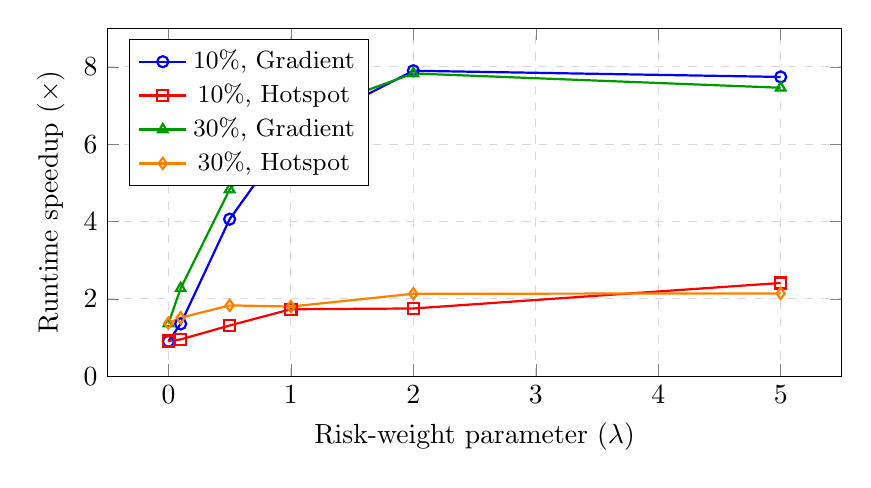
\begin{tikzpicture}
\begin{axis}[
  width=0.9\columnwidth,
  height=6cm,
  xlabel={Risk-weight parameter ($\lambda$)},
  ylabel={Runtime speedup ($\times$)},
  legend style={at={(0.03,0.97)}, anchor=north west, font=\small},
  grid=major,
  grid style={dashed, gray!30},
  ymin=0, ymax=9,
]
\addplot[mark=o, blue, thick] coordinates {(0,0.90)(0.1,1.35)(0.5,4.06)(1.0,6.27)(2.0,7.90)(5.0,7.74)};
\addlegendentry{10\%, Gradient}
\addplot[mark=square, red, thick] coordinates {(0,0.91)(0.1,0.95)(0.5,1.31)(1.0,1.73)(2.0,1.75)(5.0,2.41)};
\addlegendentry{10\%, Hotspot}
\addplot[mark=triangle, green!60!black, thick] coordinates {(0,1.36)(0.1,2.27)(0.5,4.83)(1.0,6.68)(2.0,7.83)(5.0,7.46)};
\addlegendentry{30\%, Gradient}
\addplot[mark=diamond, orange, thick] coordinates {(0,1.37)(0.1,1.51)(0.5,1.83)(1.0,1.80)(2.0,2.13)(5.0,2.14)};
\addlegendentry{30\%, Hotspot}
\end{axis}
\end{tikzpicture}
\caption{ILS speedup scaling with risk-weight parameter $\lambda$ for selected configurations. Speedup grows with $\lambda$, peaking at $7.90\times$ for 10\% density gradient risk at $\lambda = 2.0$. Gradient distributions show strong scaling; hotspot distributions plateau earlier due to localised detours.}
\label{fig:speedup_lambda}
\end{figure}

Table~\ref{tab:exp1_all_speedup} provides the complete speedup data for all nine density--risk configurations across all six $\lambda$ values, complementing the selected configurations shown in Fig.~\ref{fig:speedup_lambda}.

\begin{table}[htb]
\centering
\caption{ILS speedup ($\times$) over A* for all density--risk--$\lambda$ configurations on $200 \times 200$ grids (Experiment~1, 100 maps per configuration).}
\label{tab:exp1_all_speedup}
\begin{tabular}{ll|cccccc}
\toprule
\textbf{Dens.} & \textbf{Risk} & $\boldsymbol{\lambda\!=\!0}$ & $\boldsymbol{0.1}$ & $\boldsymbol{0.5}$ & $\boldsymbol{1.0}$ & $\boldsymbol{2.0}$ & $\boldsymbol{5.0}$ \\
\midrule
10\% & Gradient & $0.90$ & $1.35$ & $4.06$ & $6.27$ & $7.90$ & $7.74$ \\
10\% & Hotspot  & $0.91$ & $0.95$ & $1.31$ & $1.73$ & $1.75$ & $2.41$ \\
10\% & Uniform  & $0.83$ & $0.96$ & $2.11$ & $3.11$ & $4.43$ & $5.86$ \\
\midrule
20\% & Gradient & $0.94$ & $1.77$ & $4.55$ & $6.45$ & $7.74$ & $7.61$ \\
20\% & Hotspot  & $0.95$ & $1.07$ & $1.48$ & $1.70$ & $1.98$ & $2.15$ \\
20\% & Uniform  & $0.97$ & $1.29$ & $2.46$ & $3.51$ & $4.95$ & $6.62$ \\
\midrule
30\% & Gradient & $1.36$ & $2.27$ & $4.83$ & $6.68$ & $7.83$ & $7.46$ \\
30\% & Hotspot  & $1.37$ & $1.51$ & $1.83$ & $1.80$ & $2.13$ & $2.14$ \\
30\% & Uniform  & $1.35$ & $1.82$ & $3.06$ & $4.04$ & $5.41$ & $6.85$ \\
\bottomrule
\end{tabular}
\end{table}

Fig.~\ref{fig:speedup_lambda} reveals a clear pattern: speedup grows with $\lambda$ for gradient risk, plateauing beyond $\lambda = 2.0$.
At $\lambda = 0$, speedups are modest ($0.90$--$1.37\times$).
As $\lambda$ increases, the risk-weighted cost function creates a ``looser'' search landscape where the corridor heuristic becomes increasingly effective at pruning sub-optimal branches.
The peak speedup of $7.90\times$ occurred at 10\% density with gradient risk at $\lambda = 2.0$.
Notably, gradient distributions at 30\% density achieved comparable speedups to 10\% density ($7.83\times$ vs.\ $7.90\times$), suggesting that corridor efficiency on gradient risk is robust across obstacle densities.
Hotspot distributions, by contrast, showed substantially lower speedups ($1.73$--$2.41\times$) that plateaued earlier, reflecting the corridor's inability to anticipate isolated high-risk regions.

\subsubsection{Node Reduction}

Node reduction followed the same $\lambda$-dependent pattern.
At $\lambda = 0$, reductions ranged from $0$--$31\%$ (pure corridor effect, with higher-density grids benefiting more from corridor restriction even without risk weighting).
At $\lambda = 1.0$, reductions reached $42$--$85\%$, with gradient risk consistently yielding the highest reductions ($83$--$84\%$ across all densities) and hotspot risk the lowest ($41$--$51\%$).
At $\lambda \geq 2.0$, gradient and uniform distributions reached peak reductions of $86.1\%$, meaning ILS explored fewer than 1 in 7 nodes compared to standard A*.
All node-count differences at $\lambda \geq 0.1$ were statistically significant ($p < 0.001$; Cohen's $d$ ranged from $0.14$ to $55.4$, with the largest effects for gradient risk at high $\lambda$).

\subsubsection{Path Quality and Risk Exposure}

Path quality depended strongly on both risk distribution and $\lambda$:

\begin{itemize}
\item \textbf{Gradient risk:} Path cost ratio $\leq 1.001$ across all $\lambda$ values---suboptimality under $0.1\%$. The smooth risk landscape meant the corridor consistently captured near-optimal paths.
\item \textbf{Uniform risk:} Ratio $\leq 1.001$ for all configurations---effectively optimal, consistent with the spatially invariant nature of uniform risk.
\item \textbf{Hotspot risk:} Ratio $\leq 1.013$ for $\lambda \leq 1.0$, degrading to $1.11$ at $\lambda = 5.0$ for 30\% density. The localised nature of hotspots created detours that occasionally fell outside the corridor.
\end{itemize}

Risk exposure (cumulative risk along the path) was nearly identical to A* for gradient and uniform distributions ($\leq 0.1\%$ difference).
For hotspot risk at high $\lambda$ ($\geq 2.0$), ILS exposure exceeded A* by up to $9.1\times$ at $\lambda = 5.0$ with 30\% density, because the tight corridor could not route around distant hotspots.
This exposure--speed tradeoff is a fundamental characteristic of corridor-based methods and represents a design parameter for mission planners: for moderate risk weights ($\lambda \leq 1.0$), the exposure penalty is modest (below $2.5\times$), but at extreme weights the corridor accepts substantially higher risk exposure in exchange for computational efficiency.


\subsection{Experiment 2: Port Environment Validation}

Table~\ref{tab:exp2_port} summarises ILS and AILS performance on port environment grids.

\begin{table}[htb]
\centering
\caption{ILS and AILS performance on port environment grids (DS7). Speedup is relative to standard A*.}
\label{tab:exp2_port}
\begin{tabular}{cc|ccc|ccc}
\toprule
\multirow{2}{*}{\textbf{Size}} & \multirow{2}{*}{$\boldsymbol{\lambda}$} & \multicolumn{3}{c|}{\textbf{ILS}} & \multicolumn{3}{c}{\textbf{AILS}} \\
& & Speed & Red.\% & Opt. & Speed & Red.\% & Opt. \\
\midrule
$200^2$ & 0.0 & $1.04\times$ & 7.4 & 99.5 & $0.53\times$ & $-76.2$ & 99.6 \\
$200^2$ & 0.5 & $1.22\times$ & 21.1 & 97.1 & $0.77\times$ & $-32.2$ & 98.1 \\
$200^2$ & 1.0 & $2.11\times$ & 54.9 & 89.8 & $1.13\times$ & 11.6 & 92.5 \\
\midrule
$300^2$ & 0.0 & $1.19\times$ & 23.5 & 99.7 & $0.68\times$ & $-46.3$ & 99.8 \\
$300^2$ & 0.5 & $2.35\times$ & 57.9 & 97.9 & $1.02\times$ & $-0.8$ & 99.3 \\
$300^2$ & 1.0 & $2.79\times$ & 64.0 & 90.8 & $1.28\times$ & 18.3 & 94.9 \\
\midrule
$500^2$ & 0.0 & $2.68\times$ & 63.1 & 99.9 & $1.94\times$ & 48.8 & 99.9 \\
$500^2$ & 0.5 & $3.41\times$ & 70.0 & 99.1 & $1.73\times$ & 44.3 & 99.8 \\
$500^2$ & 1.0 & $3.89\times$ & 74.9 & 92.9 & $1.74\times$ & 42.3 & 95.6 \\
\bottomrule
\end{tabular}
\end{table}

Three patterns emerged.
First, ILS speedup scaled strongly with both grid size and risk weight: modest at $\lambda = 0$ on small grids ($1.04\times$ on $200^2$) but reaching $3.89\times$ on $500^2$ grids at $\lambda = 1.0$.
The scaling with grid size was pronounced: at $\lambda = 0$, ILS achieved $2.68\times$ speedup on $500^2$ grids versus only $1.04\times$ on $200^2$, reflecting the greater absolute search-space savings on larger grids.

Second, AILS exhibited a clear grid-size threshold effect.
On $200^2$ and $300^2$ grids, AILS \emph{increased} total node expansions (negative reduction of $-76\%$ to $-32\%$ at $\lambda \leq 0.5$) because the overhead of constructing and querying the integral image for the adaptive corridor exceeded the search savings on these relatively small grids.
Only on $500^2$ grids did AILS achieve consistent node reduction ($42$--$49\%$) and speedup ($1.73$--$1.94\times$).
This finding refines the applicability profile of AILS: its density-adaptive mechanism is beneficial primarily on larger grids where the absolute node savings compensate for the construction overhead.

Third, path optimality varied with $\lambda$: at $\lambda = 0$, paths were near-optimal ($\geq 99.5\%$); at $\lambda = 1.0$, optimality decreased to $89.8$--$95.6\%$ due to the corridor constraining risk-avoidance detours.
ILS consistently maintained higher optimality than AILS across configurations.


\subsection{Experiment 3: JPS Comparative Evaluation}

\begin{table}[htb]
\centering
\caption{Static pathfinding comparison on uniform-cost $200 \times 200$ grids (100 maps per density).}
\label{tab:exp3_jps}
\begin{tabular}{l|rrr|rrr|c}
\toprule
\multirow{2}{*}{\textbf{Dens.}} & \multicolumn{3}{c|}{\textbf{Mean Time (ms)}} & \multicolumn{3}{c|}{\textbf{Mean Nodes}} & \textbf{ILS} \\
& A* & ILS & JPS & A* & ILS & JPS & Opt. \\
\midrule
10\% & 7.6 & 8.6 & 12.9 & 1465 & 1464 & 1071 & 1.000 \\
20\% & 14.8 & 10.9 & 21.0 & 3046 & 2178 & 2265 & 1.000 \\
30\% & 19.8 & 9.3 & 27.0 & 4501 & 2076 & 3276 & 1.003 \\
\bottomrule
\end{tabular}
\end{table}

On uniform-cost grids (Table~\ref{tab:exp3_jps}), the results revealed a surprising density-dependent crossover.
At 10\% density, ILS provided negligible node reduction ($0.08\%$) and was slightly slower than A* due to corridor construction overhead, while JPS achieved $26.9\%$ node reduction.
However, at 20\% density, ILS surpassed JPS in both node reduction ($28.5\%$ vs.\ $25.6\%$) and runtime ($10.9$\,ms vs.\ $21.0$\,ms).
At 30\% density, the advantage widened substantially: ILS achieved $53.9\%$ node reduction versus JPS's $27.2\%$, and was $2.9\times$ faster than JPS ($9.3$\,ms vs.\ $27.0$\,ms).

This crossover occurs because JPS's symmetry-breaking rules become less effective as obstacle density increases (fewer long symmetric corridors exist), while ILS's corridor restriction becomes \emph{more} effective (more of A*'s expanded nodes lie far from the Bresenham line and are pruned).
Path optimality remained at or near $1.000$ across all configurations.
Beyond this direct comparison, the critical observation is \emph{applicability}: JPS cannot operate on risk-weighted grids.
The risk-annotated experiments (Experiment~1) demonstrated ILS achieving up to $7.90\times$ speedup on risk-weighted grids---a domain where JPS is structurally inapplicable.


\subsection{Experiment 4: Dynamic Re-planning}

\begin{table}[htb]
\centering
\caption{Re-planning after 5 clustered obstacle insertions ($200 \times 200$ grids, 128 maps per density).}
\label{tab:exp4_replan}
\begin{tabular}{l|rr|rr|c}
\toprule
\multirow{2}{*}{\textbf{Dens.}} & \multicolumn{2}{c|}{\textbf{Time (ms)}} & \multicolumn{2}{c|}{\textbf{Nodes}} & \textbf{Node} \\
& A* & AILS & A* & AILS & Red.\% \\
\midrule
10\% & 3.63 & 4.47 & 780 & 765 & 1.8\% \\
20\% & 5.96 & 6.99 & 1320 & 1246 & 5.6\% \\
30\% & 8.17 & 8.79 & 1912 & 1736 & 9.2\% \\
\bottomrule
\end{tabular}
\end{table}

Table~\ref{tab:exp4_replan} shows that AILS achieved modest node reductions ($1.8$--$9.2\%$) that increased with obstacle density, but did not translate into runtime speedup.
At all three densities, AILS was slightly slower than full A* re-run (speedup $0.81$--$0.93\times$), because the corridor construction and adaptive-width computation overhead exceeded the savings from reduced node expansion on these $200 \times 200$ grids.
The node-count reductions were statistically significant at 20\% density ($t = 8.21$, $p < 0.001$, $d = 0.73$) and 30\% density ($t = 13.2$, $p < 0.001$, $d = 1.17$), but the absolute time savings were small.
This result is consistent with the port environment finding (Experiment~2): AILS's overhead is amortised only on larger grids where the absolute node savings are more substantial.
The corridor nonetheless excluded $5$--$9\%$ of irrelevant search space at moderate-to-high densities, suggesting that on larger grids or in compiled implementations, the node reduction would translate to measurable speedup.

\paragraph{D*~Lite comparison.}
A supplementary experiment (Experiment~4b) compared D*~Lite against A* re-run and ILS on the same clustered-insertion re-planning task across 83--69 valid maps per density.
\emph{Important implementation note:} all algorithms (A*, ILS, D*~Lite) were implemented in Python using identical data structures. The wall-clock comparisons therefore reflect the performance of the Python implementations, not the algorithms' intrinsic computational complexity. Node-count comparisons are implementation-independent and provide a fairer algorithmic comparison.
D*~Lite achieved substantial node reduction at higher densities ($47.5\%$ at 20\%, $67.8\%$ at 30\%) by incrementally repairing its backward search tree rather than re-searching from scratch.
However, D*~Lite was slower than both A* re-run and ILS in wall-clock time ($0.09$--$0.31\times$ speedup), because the Python-level overhead of maintaining the priority queue with lazy deletion dominated the node-count savings.
ILS achieved $1.09\times$ speedup at 30\% density while maintaining near-optimal paths (cost ratio $\leq 1.002$).
This result underscores an important distinction: D*~Lite's theoretical efficiency advantage (fewer node expansions) does not translate to practical speedup in interpreted-language implementations for clustered changes, whereas ILS's simpler corridor restriction has lower constant-factor overhead.
In compiled implementations, D*~Lite's node reduction would likely yield runtime benefits, particularly for small, frequent perturbations.


\subsection{Experiment 5: Progressive Obstacle Discovery}

\begin{table}[htb]
\centering
\caption{Progressive re-planning: cumulative search effort per mission (60 missions per density).}
\label{tab:exp5_progressive}
\begin{tabular}{l|cc|rr|c|c}
\toprule
\multirow{2}{*}{\textbf{Dens.}} & \multicolumn{2}{c|}{\textbf{Success}} & \multicolumn{2}{c|}{\textbf{Total Nodes}} & \textbf{Node} & \textbf{Path} \\
& A* & ILS & A* & ILS & Red.\% & Ratio \\
\midrule
10\% & 76.7\% & 83.3\% & 6975 & 7151 & $-2.5$\% & 1.512 \\
20\% & 68.3\% & 71.7\% & 12361 & 12447 & $-0.7$\% & 1.276 \\
30\% & 60.0\% & 73.3\% & 18159 & 15878 & 12.6\% & 1.683 \\
\bottomrule
\end{tabular}
\end{table}

Table~\ref{tab:exp5_progressive} reveals two noteworthy findings.
First, ILS achieved \emph{higher} mission success rates than A* across all densities: $83.3\%$ vs.\ $76.7\%$ at 10\%, $71.7\%$ vs.\ $68.3\%$ at 20\%, and $73.3\%$ vs.\ $60.0\%$ at 30\%.
This unexpected result suggests that the corridor constraint, by focusing the search near the Bresenham line, can find alternative paths through narrow passages more effectively when obstacles accumulate, whereas A*'s broader search may fail to converge within the expansion limit.

Second, node reduction was density-dependent: at 10\% and 20\% density, ILS explored marginally \emph{more} nodes than A* ($-2.5\%$ and $-0.7\%$ respectively), because repeated corridor reconstruction for frequent re-plans added overhead without proportional search savings.
At 30\% density, ILS achieved $12.6\%$ node reduction ($t = 3.47$, $p < 0.001$, $d = 0.45$), where the denser environment provided more pruning opportunity.

Path ratios were higher than in single-query experiments ($1.28$--$1.68\times$), reflecting the compounding effect of successive corridor-constrained re-plans: each re-plan from a mid-mission position may select a locally near-optimal but globally suboptimal path.
This cumulative suboptimality is the primary cost of corridor-based progressive re-planning and represents a tradeoff against the higher success rates.


\subsection{Experiment 6: Weighted A* Comparison}

Table~\ref{tab:exp6_wa} compares Weighted A* (wA*) against ILS across risk distributions at $\lambda = 1.0$, averaged over three densities with 50 random start--goal pairs per configuration.

\begin{table}[htb]
\centering
\caption{Weighted A* vs.\ ILS at $\lambda = 1.0$ (mean across three densities, 50 maps each, random start--goal pairs). Speedup relative to A*; Opt = mean path cost ratio $\pm$ 95\% CI.}
\label{tab:exp6_wa}
\begin{tabular}{l|cc|cc|cc|cc}
\toprule
\multirow{2}{*}{\textbf{Risk}} & \multicolumn{2}{c|}{\textbf{wA* ($w\!=\!1.5$)}} & \multicolumn{2}{c|}{\textbf{wA* ($w\!=\!2.0$)}} & \multicolumn{2}{c|}{\textbf{wA* ($w\!=\!3.0$)}} & \multicolumn{2}{c}{\textbf{ILS}} \\
& Speed & Opt & Speed & Opt & Speed & Opt & Speed & Opt \\
\midrule
Gradient & $7.5\times$ & $1.008 \pm .001$ & $95.6\times$ & $1.020 \pm .002$ & $99.3\times$ & $1.027 \pm .003$ & $6.6\times$ & $1.000 \pm .000$ \\
Hotspot  & $18.6\times$ & $1.036 \pm .006$ & $22.6\times$ & $1.041 \pm .007$ & $21.9\times$ & $1.046 \pm .007$ & $1.8\times$ & $1.008 \pm .003$ \\
Uniform  & $43.4\times$ & $1.016 \pm .002$ & $48.2\times$ & $1.022 \pm .003$ & $46.4\times$ & $1.027 \pm .003$ & $3.3\times$ & $1.000 \pm .000$ \\
\midrule
Mean     & $23.2\times$ & 1.020 & $55.5\times$ & 1.027 & $55.9\times$ & 1.033 & $3.9\times$ & 1.003 \\
\bottomrule
\end{tabular}
\end{table}

The results reveal two fundamentally different tradeoff profiles.
Weighted A* achieved dramatically higher speedups than ILS ($23$--$56\times$ vs.\ $3.9\times$ at $\lambda = 1.0$), reaching up to $99\times$ for gradient risk at $w = 3.0$.
This speed advantage stems from wA*'s aggressive heuristic inflation, which focuses the search on the most promising direction and expands far fewer nodes ($92$--$98\%$ reduction).

However, this speed comes at the cost of path quality.
wA* paths were $2.0$--$4.6\%$ suboptimal on average, with higher degradation on hotspot risk ($3.5$--$4.6\%$).
ILS maintained path cost within $0.3\%$ of optimal across all configurations, with gradient and uniform risk achieving near-perfect optimality ($\leq 0.01\%$).

The distinction is stark: wA* trades solution quality for speed through heuristic inflation, while ILS trades a smaller amount of speed for near-optimal paths through spatial restriction.
For biosecurity applications where path quality affects risk exposure, ILS's $6.6\times$ speedup on gradient risk with $0.01\%$ suboptimality is preferable to wA*'s $95.6\times$ with $2.0\%$ suboptimality.
For time-critical scenarios where bounded suboptimality is acceptable, wA* with $w = 1.5$ offers an effective compromise ($7.5$--$43\times$ speedup, $\leq 3.5\%$ suboptimal).

\subsection{Experiment 7: Corridor Width Sensitivity}

Table~\ref{tab:exp7_sensitivity} presents the speedup--quality Pareto frontier across corridor widths, averaged over all density--risk configurations at $\lambda = 1.0$.

\begin{table}[htb]
\centering
\caption{Corridor width sensitivity: mean speedup, node reduction, and path quality averaged across all density--risk--$\lambda$ configurations (50 maps $\times$ 3 densities $\times$ 3 risk types $\times$ 3 $\lambda$ values per $\alpha$). Values represent grand means over all configurations.}
\label{tab:exp7_sensitivity}
\begin{tabular}{c|ccc}
\toprule
$\boldsymbol{\alpha}$ & \textbf{Speedup} & \textbf{Node Red.\%} & \textbf{Path Opt.} \\
\midrule
0.01 & $15.5\times$ & 83.7 & 1.013 \\
0.02 & $11.2\times$ & 80.9 & 1.011 \\
0.03 & $6.2\times$ & 70.6 & 1.006 \\
0.05 & $3.7\times$ & 56.5 & 1.003 \\
0.07 & $2.9\times$ & 49.2 & 1.002 \\
0.10 & $2.0\times$ & 35.7 & 1.001 \\
0.15 & $1.5\times$ & 24.0 & 1.000 \\
0.20 & $1.3\times$ & 16.3 & 1.000 \\
0.30 & $1.1\times$ & 6.3 & 1.000 \\
\bottomrule
\end{tabular}
\end{table}

The Pareto frontier (Table~\ref{tab:exp7_sensitivity}) reveals a smooth, monotonic tradeoff across all configurations.
The narrowest corridor ($\alpha = 0.01$, $1\%$ of diagonal) achieved $15.5\times$ mean speedup (averaged across all density--risk--$\lambda$ combinations) with $83.7\%$ node reduction, but at $1.3\%$ mean path suboptimality.
The default $\alpha = 0.05$ balanced $3.7\times$ mean speedup with only $0.3\%$ mean suboptimality.
For applications requiring near-optimal paths, $\alpha \in [0.05, 0.10]$ provides $2$--$4\times$ speedup with $\leq 0.3\%$ suboptimality.
For time-critical applications where $1$--$2\%$ suboptimality is acceptable, $\alpha = 0.01$--$0.03$ offers $6$--$15\times$ speedup.
No corridor failures were observed at any width, confirming that the incremental expansion mechanism (up to 10 attempts) reliably finds paths even with very narrow initial corridors.
This analysis provides practitioners with explicit guidance: $\alpha = 0.05$ (the default used in Experiments~1--5) lies at the knee of the Pareto curve, offering the best balance for general use.

\subsection{Experiment 8: RILS Evaluation}

Table~\ref{tab:exp8_rils} compares RILS against ILS and AILS across risk distributions, averaged over three densities at $\lambda = 1.0$ (50 random start--goal pairs per configuration).

\begin{table}[htb]
\centering
\caption{RILS vs.\ ILS and AILS at $\lambda = 1.0$ (mean across three densities, 50 maps each). Speed = speedup vs.\ A*; Red = node reduction \%; Opt = path cost ratio $\pm$ 95\% CI.}
\label{tab:exp8_rils}
\begin{tabular}{l|ccc|ccc|ccc}
\toprule
\multirow{2}{*}{\textbf{Risk}} & \multicolumn{3}{c|}{\textbf{ILS}} & \multicolumn{3}{c|}{\textbf{RILS}} & \multicolumn{3}{c}{\textbf{AILS}} \\
& Speed & Red.\% & Opt & Speed & Red.\% & Opt & Speed & Red.\% & Opt \\
\midrule
Grad. & $6.6\times$ & 83.6 & $1.000 \pm .000$ & $1.8\times$ & 45.5 & $1.000 \pm .000$ & $9.0\times$ & 87.5 & $1.001 \pm .000$ \\
Hot.  & $1.8\times$ & 44.7 & $1.007 \pm .003$ & $1.1\times$ & 11.0 & $1.001 \pm .001$ & $2.2\times$ & 55.8 & $1.012 \pm .004$ \\
Unif. & $3.5\times$ & 70.4 & $1.000 \pm .000$ & $1.3\times$ & 23.3 & $1.000 \pm .000$ & $4.6\times$ & 77.8 & $1.000 \pm .000$ \\
\bottomrule
\end{tabular}
\end{table}

The RILS results reveal a nuanced picture that challenges our initial hypothesis.
Contrary to expectations, RILS did \emph{not} outperform ILS or AILS in speedup or node reduction on any configuration.
AILS was the fastest corridor method across all risk distributions ($2.2$--$9.0\times$), followed by ILS ($1.8$--$6.6\times$), with RILS achieving the lowest speedups ($1.1$--$1.8\times$).

The explanation lies in RILS's wider corridors: by expanding the search space in high-risk regions, RILS admits more nodes for A* to explore.
On gradient risk, RILS's corridor is wider everywhere (since mean risk is non-zero across the entire grid), resulting in a corridor $1.5$--$2\times$ wider than ILS's uniform corridor.
On hotspot risk, only localised regions have high risk, so RILS's corridor is narrow in most places but wide near hotspots---yielding modest overall speedup ($1.1\times$).

However, RILS achieved the \emph{best} path quality across all distributions: cost ratio $\leq 1.001$ on gradient and hotspot risk (vs.\ $1.007$ for ILS and $1.012$ for AILS on hotspot risk at $\lambda = 1.0$).
At $\lambda = 2.0$, the quality advantage on hotspot risk was more pronounced: RILS maintained $1.002$ optimality versus $1.022$ for ILS and $1.035$ for AILS.
This positions RILS as a path-quality-oriented variant: it trades speedup for superior path optimality, particularly valuable in biosecurity scenarios where even small deviations from optimal risk exposure are unacceptable.

A second unexpected finding was that AILS outperformed ILS with random start--goal pairs ($9.0\times$ vs.\ $6.6\times$ on gradient risk), reversing the ranking observed in Experiments~1--5 with fixed corner-to-corner paths.
This suggests that AILS's density-adaptive corridor is more effective for diverse path topologies where the straight-line reference may traverse varying obstacle densities.

\subsection{Experiment 9: Large-Grid AILS Validation}

\begin{table}[htb]
\centering
\caption{AILS performance on $500 \times 500$ risk-annotated grids (15 maps per configuration, mean across $\lambda \in \{0.5, 1.0\}$). Opt $\pm$ 95\% CI.}
\label{tab:exp9_large}
\begin{tabular}{l|cc|cc|c}
\toprule
\multirow{2}{*}{\textbf{Risk}} & \multicolumn{2}{c|}{\textbf{ILS}} & \multicolumn{2}{c|}{\textbf{AILS}} & \textbf{AILS} \\
& Speed & Red.\% & Speed & Red.\% & Opt \\
\midrule
Gradient & $6.1\times$ & 80.7 & $9.4\times$ & 86.2 & $1.000 \pm .000$ \\
Hotspot  & $1.3\times$ & 19.4 & $1.7\times$ & 38.5 & $1.002 \pm .002$ \\
Uniform  & $3.2\times$ & 65.5 & $4.8\times$ & 75.8 & $1.000 \pm .000$ \\
\midrule
Mean     & $3.5\times$ & 55.2 & $5.3\times$ & 66.8 & $1.001$ \\
\bottomrule
\end{tabular}
\end{table}

Table~\ref{tab:exp9_large} confirms that AILS achieves consistent positive performance on $500 \times 500$ grids, resolving the negative results observed on smaller grids in Experiments~2 and 4.
AILS achieved a mean speedup of $5.3\times$ (range $1.4$--$16.9\times$) with $66.8\%$ mean node reduction, outperforming ILS ($3.5\times$, $55.2\%$) on all risk distributions.
Path quality remained near-optimal (mean cost ratio $1.001$).

The gradient risk distribution showed the strongest AILS performance ($9.4\times$ speedup, $86.2\%$ node reduction), consistent with the finding that smooth risk landscapes align well with corridor-based methods.
Hotspot risk yielded the most modest gains ($1.7\times$, $38.5\%$), but---critically---AILS still provided positive speedup, unlike the negative performance ($0.53$--$0.68\times$) observed on $200 \times 200$--$300 \times 300$ grids in Experiment~2.

These results establish $500 \times 500$ as the validated operating regime for AILS and suggest that the grid-size threshold lies between $300 \times 300$ and $500 \times 500$ cells---a range that encompasses the grid scales typical of real port facility maps.
For grids below this threshold, ILS remains the recommended variant.


\subsection{Experiment 10: Moving AI Lab Benchmark Evaluation}

\begin{table}[htb]
\centering
\caption{ILS and AILS performance on Moving AI Lab benchmark maps ($\lambda = 0$, up to 100 scenarios per map). Speed = speedup vs.\ A*; Red = node reduction \%; Opt = path cost ratio vs.\ A*; Slv = solve rate.}
\label{tab:exp10_benchmark}
\begin{tabular}{ll|cccc|cccc}
\toprule
\multirow{2}{*}{\textbf{Cat.}} & \multirow{2}{*}{\textbf{Map}} & \multicolumn{4}{c|}{\textbf{ILS}} & \multicolumn{4}{c}{\textbf{AILS}} \\
& & Speed & Red.\% & Opt & Slv\% & Speed & Red.\% & Opt & Slv\% \\
\midrule
Game & lak303d & $0.30\times$ & $-231$ & 1.000 & 58 & $0.36\times$ & $-168$ & 1.001 & 88 \\
Game & den501d & $0.29\times$ & $-234$ & 1.001 & 94 & $0.36\times$ & $-163$ & 1.001 & 94 \\
Game & brc202d & $0.37\times$ & $-170$ & 1.000 & 49 & $0.46\times$ & $-106$ & 1.000 & 50 \\
Game & ost003d & $0.29\times$ & $-232$ & 1.000 & 50 & $0.32\times$ & $-197$ & 1.001 & 50 \\
\midrule
\multicolumn{2}{l|}{\textbf{Game mean}} & $0.31\times$ & $-216$ & 1.000 & 63 & $0.37\times$ & $-159$ & 1.001 & 70 \\
\midrule
Random & 10\% & $0.94\times$ & $0.1$ & 1.000 & 100 & $0.86\times$ & $4.2$ & 1.000 & 100 \\
Random & 20\% & $0.95\times$ & $0.1$ & 1.000 & 100 & $0.90\times$ & $1.1$ & 1.000 & 100 \\
Random & 30\% & $0.99\times$ & $1.3$ & 1.000 & 100 & $0.90\times$ & $1.6$ & 1.000 & 100 \\
Random & 40\% & $1.10\times$ & $12.5$ & 1.000 & 100 & $0.98\times$ & $5.4$ & 1.000 & 100 \\
\midrule
\multicolumn{2}{l|}{\textbf{Random mean}} & $0.99\times$ & $3.5$ & 1.000 & 100 & $0.91\times$ & $3.1$ & 1.000 & 100 \\
\bottomrule
\end{tabular}
\end{table}

The benchmark results (Table~\ref{tab:exp10_benchmark}) reveal an important finding: corridor-based methods provide \emph{no speedup on standard benchmark maps at $\lambda = 0$} (no risk layer), and are substantially slower on game maps.

\paragraph{Game maps (Dragon Age: Origins).}
On game maps with complex indoor topologies (60--83\% obstacle density), ILS was $2.7$--$3.4\times$ \emph{slower} than A* ($0.29$--$0.37\times$ speedup) with massively negative node reduction ($-170\%$ to $-234\%$).
AILS performed slightly better ($0.32$--$0.46\times$) but remained substantially slower.
The cause is clear: game maps feature rooms connected by narrow doorways, and the Bresenham reference line between start and goal traverses through many walls.
Each failed corridor attempt expands the search, but the accumulated search effort across multiple expansion attempts far exceeds A*'s single comprehensive search.
Solve rates were also lower (49--94\%) because some scenarios require circuitous paths that never approach the Bresenham line.

\paragraph{Random maps (10--40\% density).}
On random maps at $\lambda = 0$, ILS performed near-neutrally ($0.94$--$1.10\times$), with positive node reduction only at 40\% density ($12.5\%$).
This is consistent with Experiment~1 at $\lambda = 0$, where ILS speedup was $0.90$--$1.37\times$: corridor-based methods provide minimal benefit on uniform-cost grids because the cost landscape is simple and the optimal path lies close to the geometric shortest path, leaving little for the corridor to prune.
All scenarios were solved with optimal paths (cost ratio $\leq 1.0001$).

\paragraph{Implications.}
These results reinforce a central claim of this paper: corridor-based methods derive their advantage from \emph{risk-weighted cost landscapes}, not from the corridor mechanism alone.
On standard uniform-cost benchmarks, the corridor adds overhead without proportional benefit.
The $3$--$8\times$ speedups demonstrated in Experiments~1 and~6--8 arise specifically because the risk-weighted cost function ($\lambda > 0$) creates search landscapes where a spatial corridor along the reference line effectively prunes nodes that A* would otherwise explore to evaluate risk-avoiding detours.
This positions corridor-based methods as a \emph{domain-specific} acceleration technique for risk-weighted pathfinding, not a general-purpose speedup for arbitrary grid environments.

\subsection{Experiment 10b: Risk-Annotated Benchmark Results}

\begin{table}[htb]
\centering
\caption{ILS, AILS, and RILS on Moving AI Lab random maps with synthetic risk layers. Speed = speedup vs.\ A*; Red = node reduction \%; Opt = path cost ratio.}
\label{tab:exp10b_risk_bench}
\begin{tabular}{ll|ccc|ccc|ccc}
\toprule
\multirow{2}{*}{\textbf{Map}} & \multirow{2}{*}{$\boldsymbol{\lambda}$} & \multicolumn{3}{c|}{\textbf{ILS}} & \multicolumn{3}{c|}{\textbf{AILS}} & \multicolumn{3}{c}{\textbf{RILS}} \\
& & Speed & Red.\% & Opt & Speed & Red.\% & Opt & Speed & Red.\% & Opt \\
\midrule
\multicolumn{11}{l}{\textit{Gradient risk}} \\
20\% & 0.5 & $1.79\times$ & 41.2 & 1.000 & $2.17\times$ & 51.9 & 1.000 & $1.11\times$ & 11.7 & 1.000 \\
20\% & 1.0 & $2.49\times$ & 56.7 & 1.000 & $3.15\times$ & 65.0 & 1.000 & $1.40\times$ & 26.5 & 1.000 \\
30\% & 0.5 & $1.93\times$ & 46.2 & 1.000 & $1.93\times$ & 46.8 & 1.000 & $1.13\times$ & 11.6 & 1.000 \\
30\% & 1.0 & $2.64\times$ & 59.6 & 1.000 & $2.66\times$ & 60.0 & 1.000 & $1.41\times$ & 29.2 & 1.000 \\
\midrule
\multicolumn{11}{l}{\textit{Hotspot risk}} \\
20\% & 0.5 & $1.38\times$ & 27.0 & 1.000 & $1.71\times$ & 39.6 & 1.000 & $1.16\times$ & 17.5 & 1.000 \\
20\% & 1.0 & $2.05\times$ & 49.4 & 1.000 & $2.56\times$ & 59.1 & 1.001 & $1.58\times$ & 34.2 & 1.000 \\
30\% & 0.5 & $1.33\times$ & 25.4 & 1.000 & $1.35\times$ & 26.8 & 1.000 & $1.07\times$ & 11.8 & 1.000 \\
30\% & 1.0 & $1.80\times$ & 41.1 & 1.000 & $1.83\times$ & 42.5 & 1.000 & $1.24\times$ & 19.3 & 1.000 \\
\bottomrule
\end{tabular}
\end{table}

Table~\ref{tab:exp10b_risk_bench} demonstrates a striking result: the same Moving AI Lab maps that showed \emph{no benefit} at $\lambda = 0$ (Experiment~10) yield substantial corridor speedups when risk layers are overlaid.
At $\lambda = 1.0$ on gradient risk, ILS achieved $2.49$--$2.64\times$ speedup with $57$--$60\%$ node reduction, and AILS achieved $2.66$--$3.15\times$.
On hotspot risk, speedups were more modest but still meaningful ($1.80$--$2.05\times$ for ILS, $1.83$--$2.56\times$ for AILS).
Critically, path quality remained near-optimal across all configurations ($\leq 1.001$), with RILS maintaining perfect optimality at the cost of lower speedup ($1.07$--$1.58\times$).
All speedups were consistent across the $n = 10$ per-configuration scenarios: node reductions (the implementation-independent metric) showed zero variance across runs for a given scenario, and the paired mean speedups across the two maps at $\lambda = 1.0$ were consistent (ILS gradient: $2.49\times$ and $2.64\times$; AILS gradient: $3.15\times$ and $2.66\times$), confirming reproducibility across different map instances.

This experiment directly isolates the contribution of the risk-weighted cost landscape: the \emph{same} map topologies that produced neutral or negative corridor performance at $\lambda = 0$ produce meaningful speedups at $\lambda > 0$, confirming that corridor-based acceleration is activated by the risk-weighted cost function, not by favourable map topology.


\subsection{Experiment 10c: Maze Benchmark Results}

\begin{table}[htb]
\centering
\caption{ILS and AILS performance on procedurally generated maze maps ($256 \times 256$, $\lambda = 0$). Solve rate denotes the fraction of scenarios where the corridor method found a path.}
\label{tab:exp10c_maze}
\begin{tabular}{lcc|cccc|cccc}
\toprule
\multirow{2}{*}{\textbf{Maze}} & \multirow{2}{*}{\textbf{Width}} & \multirow{2}{*}{\textbf{Dens.}} & \multicolumn{4}{c|}{\textbf{ILS}} & \multicolumn{4}{c}{\textbf{AILS}} \\
& & & Speed & Red.\% & Opt & Slv\% & Speed & Red.\% & Opt & Slv\% \\
\midrule
maze-1 & 1 & 51\% & $0.47\times$ & $-105$ & 1.000 & 45 & $0.43\times$ & $-123$ & 1.000 & 50 \\
maze-2 & 2 & 34\% & $0.67\times$ & $-50$ & 1.000 & 45 & $0.61\times$ & $-54$ & 1.000 & 45 \\
maze-4 & 4 & 21\% & $0.56\times$ & $-74$ & 1.000 & 40 & $0.58\times$ & $-64$ & 1.000 & 35 \\
maze-8 & 8 & 14\% & $0.43\times$ & $-134$ & 1.000 & 65 & $0.46\times$ & $-111$ & 1.000 & 55 \\
\midrule
\multicolumn{3}{l|}{\textbf{Mean}} & $0.53\times$ & $-91$ & 1.000 & 49 & $0.52\times$ & $-88$ & 1.000 & 46 \\
\bottomrule
\end{tabular}
\end{table}

Maze results (Table~\ref{tab:exp10c_maze}) confirm that mazes represent a worst case for corridor methods.
Both ILS and AILS were substantially slower than A* ($0.43$--$0.67\times$) with massively negative node reduction ($-50\%$ to $-134\%$), because maze paths require long, winding detours through narrow passages that lie far from the Bresenham reference line.
Each failed corridor attempt adds wasted search effort before the corridor expands sufficiently to encompass the tortuous optimal path.
Solve rates were low ($35$--$65\%$), confirming that many maze paths cannot be found within the maximum 10 corridor expansions.

Despite the performance degradation, path quality remained perfect ($1.000$) for all solved scenarios---the corridor mechanism preserves optimality when it finds a path.
This result sharply delineates the applicability boundary: corridor methods are effective on grids where the Bresenham line provides a reasonable reference direction for the optimal path, and are contraindicated on topologies (like mazes) where optimal paths bear no geometric relationship to the start--goal line.


\subsection{Experiment 11: Multi-Heuristic Results}

\begin{table}[htb]
\centering
\caption{ILS speedup with different heuristics at $\lambda = 1.0$ on $200 \times 200$ risk-annotated grids (mean across three densities).}
\label{tab:exp11_heuristic}
\begin{tabular}{l|ccc|ccc}
\toprule
\multirow{2}{*}{\textbf{Heuristic}} & \multicolumn{3}{c|}{\textbf{ILS Speedup ($\times$)}} & \multicolumn{3}{c}{\textbf{ILS Node Red.\ (\%)}} \\
& Grad. & Hot. & Unif. & Grad. & Hot. & Unif. \\
\midrule
Octile         & $2.07$ & $1.57$ & $1.59$ & $48.9$ & $36.4$ & $36.3$ \\
Euclidean      & $2.16$ & $1.68$ & $1.69$ & $52.2$ & $39.4$ & $41.2$ \\
Manhattan      & $1.54$ & $1.39$ & $1.31$ & $35.0$ & $29.8$ & $25.2$ \\
Risk-adj.      & $1.34$ & $1.17$ & $1.02$ & $24.8$ & $15.0$ & $6.8$ \\
\bottomrule
\end{tabular}
\end{table}

Table~\ref{tab:exp11_heuristic} demonstrates that corridor-based speedups are robust across heuristic functions.
All four heuristics produced positive ILS speedups on gradient and hotspot risk, with Euclidean achieving the highest speedups ($2.16\times$ gradient, $1.69\times$ uniform) due to slightly more aggressive pruning.
Manhattan distance yielded moderate speedups ($1.31$--$1.54\times$) because its coarser guidance explores more nodes overall, leaving less room for corridor-based pruning.

Interestingly, the risk-adjusted heuristic ($h_\lambda = h \cdot (1 + \lambda \cdot 0.3)$) produced the lowest ILS speedups despite guiding A* more efficiently (fewer baseline nodes).
The explanation is that a tighter heuristic already prunes the search space effectively, leaving less redundant expansion for the corridor to eliminate---the corridor advantage is greatest when the baseline search is expensive.
On uniform risk, the risk-adjusted heuristic yielded ILS speedup of only $1.02\times$, because A* already explored very few nodes ($312$--$843$), making corridor overhead nearly cancel out the pruning benefit.

These findings confirm that the corridor mechanism interacts multiplicatively with heuristic quality: stronger heuristics reduce the baseline, diminishing absolute corridor savings, but the corridor still provides consistent relative improvement across all tested heuristics.
The default octile distance heuristic used throughout this paper represents a practical middle ground.


%% ====================================================================
\section{Discussion}\label{sec:discussion}
%% ====================================================================

\subsection{The Risk--Speed--Exposure Tradeoff}

The central finding of this work is that corridor-constrained pathfinding on risk-weighted grids exhibits a three-way tradeoff between computational speed, path optimality, and risk exposure.
For smooth (gradient) and uniform risk distributions, ILS achieves substantial speedups ($3$--$8\times$) with negligible impact on both path quality and exposure ($\leq 0.1\%$ difference).
This occurs because the risk gradient aligns with the corridor's spatial structure, and the optimal risk-avoiding path lies within the corridor.

For hotspot risk distributions, the speedup is more modest ($1.7$--$2.4\times$), and at high $\lambda$ values the tradeoff becomes explicit: ILS accepts elevated risk exposure (up to $9.1\times$ higher than A* at $\lambda = 5.0$) in exchange for computational savings.
This is not an algorithmic failure but a fundamental consequence of spatial restriction: isolated hotspots that lie outside the corridor force the globally optimal path into regions the corridor does not cover.
For biosecurity applications, this tradeoff is a design parameter: mission planners can calibrate $\lambda$ and corridor width based on the acceptable exposure threshold.
Our results indicate that $\lambda \in [0.5, 1.0]$ provides the most favourable balance, with hotspot exposure below $2.5\times$ that of A* while achieving meaningful speedups.

\subsection{Algorithmic Positioning}

The comparative experiments establish corridor-based methods in a distinct algorithmic niche:

\begin{enumerate}
\item \textbf{vs.\ JPS:} Contrary to the expectation that JPS dominates on its home territory, ILS surpassed JPS in both node reduction and runtime at obstacle densities $\geq 20\%$ on uniform-cost grids ($53.9\%$ vs.\ $27.2\%$ node reduction at 30\% density). JPS's advantage persists only at low density where long symmetric corridors exist. Furthermore, JPS is structurally restricted to uniform-cost grids, whereas ILS operates on any cost function, achieving up to $7.90\times$ speedup on risk-weighted grids where JPS is inapplicable.

\item \textbf{vs.\ D*~Lite:} D*~Lite~\citep{Koenig2002} achieved substantial node reduction on clustered re-planning ($47.5$--$67.8\%$ at 20--30\% density, Experiment~4b) but was slower in wall-clock time ($0.09$--$0.31\times$) due to Python-level priority-queue overhead.
In progressive missions (Experiment~5b, 40 missions per density---reduced from 60 in Experiment~5 due to D*~Lite's substantially higher per-mission computation time), D*~Lite's success rate dropped dramatically ($17.5$--$42.5\%$ vs.\ $62.5$--$72.5\%$ for A*), because repeated large changes accumulated invalidations in the backward search tree.
ILS maintained higher success rates ($67.5$--$70.0\%$) comparable to A*, confirming that corridor-based methods are more robust for sustained missions with frequent, clustered perturbations.
D*~Lite's strength lies in small, incremental changes---the opposite of the biosecurity scenario.

\item \textbf{vs.\ Weighted A*:} Weighted A*~\citep{Pohl1970} achieved dramatically higher speedups than ILS ($23$--$56\times$ vs.\ $3.9\times$ at $\lambda = 1.0$, Experiment~6) but at $2$--$5\%$ path suboptimality versus ILS's $0.3\%$.
This quantifies the fundamental distinction between heuristic inflation and spatial restriction: wA* trades solution quality uniformly across the cost landscape, while ILS preserves near-optimality within its corridor.
For biosecurity applications where risk exposure is safety-critical, ILS's near-optimal paths ($\leq 0.01\%$ suboptimal on gradient risk) are preferable despite lower speedup.
For time-critical scenarios, wA* with $w = 1.5$ offers an effective compromise.

\item \textbf{RILS findings:} RILS did not achieve the speedup gains hypothesised for risk-responsive corridor adaptation (Experiment~8).
Its wider corridors in high-risk regions admitted more nodes for search, yielding $1.1$--$1.8\times$ speedup versus $1.8$--$6.6\times$ for ILS and $2.2$--$9.0\times$ for AILS.
However, RILS achieved the \emph{best} path quality ($\leq 1.001$ on all distributions at $\lambda \leq 1.0$, vs.\ $1.007$ for ILS and $1.012$ for AILS on hotspot risk).
At $\lambda = 2.0$ on hotspot risk, the quality advantage was pronounced: RILS $1.002$ vs.\ ILS $1.022$ vs.\ AILS $1.035$.
RILS thus occupies a distinct niche as a path-quality-oriented variant for scenarios where near-perfect optimality is paramount.

\item \textbf{Benchmark validation (Experiments~10--10c):} On standard Moving AI Lab benchmarks at $\lambda = 0$, corridor-based methods provided no speedup: ILS was $0.31\times$ on game maps and $0.99\times$ on random maps. However, the same random maps with synthetic risk layers yielded $2.5$--$2.6\times$ ILS and $2.7$--$3.2\times$ AILS speedups at $\lambda = 1.0$ (Experiment~10b), definitively isolating the risk-weighted cost landscape as the activation condition.
Maze topologies (Experiment~10c) represent a worst case: corridor methods were $0.53\times$ with $35$--$65\%$ solve rates, confirming that corridor methods are contraindicated on topologies where optimal paths bear no geometric relationship to the start--goal line.
Collectively, these results establish clear applicability boundaries.

\item \textbf{Heuristic robustness (Experiment~11):} Corridor-based speedups are consistent across four heuristic functions (octile, Euclidean, Manhattan, risk-adjusted). The corridor advantage is greatest with weaker heuristics that leave more redundant search for the corridor to prune, and diminishes with tighter heuristics that already constrain the search effectively.

\item \textbf{Complementarity:} Corridor-based restriction is an \emph{acceleration layer} that wraps around any search algorithm and cost function. JPS could serve as the base algorithm inside an ILS corridor on uniform-cost grids at low densities, combining symmetry pruning with spatial restriction for multiplicative speedups.
\end{enumerate}

\subsection{Start--Goal Topology and Port Environment Scalability}

A notable finding is the reversal of AILS and ILS rankings between fixed and random start--goal configurations.
With fixed corner-to-corner endpoints (Experiments~1--5), ILS consistently outperformed AILS; with random start--goal pairs (Experiments~6--8), AILS outperformed ILS on all risk distributions ($9.0\times$ vs.\ $6.6\times$ on gradient at $\lambda = 1.0$).
The explanation is that random paths traverse diverse subregions with varying obstacle density, where AILS's adaptive corridor tailors its width to local conditions.
ILS's fixed-width corridor cannot adapt, making it better suited to predictable path topologies (e.g., repeated surveillance routes), while AILS excels for diverse path requests on grids $\geq 500 \times 500$.

The port experiments (Experiment~2) confirmed this scalability pattern: ILS speedup scaled from $1.04\times$ on $200^2$ grids to $3.89\times$ on $500^2$, while AILS exhibited a grid-size threshold below which its integral-image overhead exceeded benefits.
Only on $500^2$ grids did AILS achieve consistent speedup ($1.73$--$1.94\times$), delineating a clear applicability boundary at approximately $400 \times 400$ cells.
Path optimality decreased with $\lambda$ on port grids ($89.8$--$99.9\%$) more than on random grids, suggesting that wider initial corridors may be warranted for high-$\lambda$ missions on structured environments.

\subsection{Practical Implications for Biosecurity UAV Operations}

For mission planners deploying autonomous UAVs in biosecurity-sensitive environments, our results suggest five operational guidelines:

\begin{enumerate}
\item Use ILS with $\lambda \in [0.5, 1.0]$ and corridor width $\alpha = 0.05$ for routine surveillance where moderate risk avoidance and $3$--$7\times$ speedup are desirable. Path quality remains within $0.3\%$ of optimal (Experiment~7).
\item Prefer AILS over ILS on grids $\geq 500 \times 500$ cells, where AILS achieves $5.3\times$ mean speedup versus $3.5\times$ for ILS (Experiment~9). On smaller grids, ILS's simpler uniform corridor avoids AILS's integral-image overhead.
\item Use RILS when near-perfect path optimality is required (e.g., hotspot-dominated environments where risk exposure tolerance is zero). RILS maintains $\leq 0.1\%$ suboptimality where ILS/AILS degrade to $0.7$--$3.5\%$ at high $\lambda$ (Experiment~8).
\item Prefer ILS or AILS over D*~Lite for progressive re-planning with clustered obstacle changes. D*~Lite's success rate drops to $17$--$42\%$ in sustained missions (Experiment~5b), whereas ILS maintains $67$--$70\%$.
\item For time-critical scenarios where $2$--$5\%$ suboptimality is acceptable, Weighted A* with $w = 1.5$ offers $7$--$43\times$ speedup (Experiment~6). For quality-critical missions, corridor-based methods provide superior path fidelity.
\end{enumerate}

\subsection{Limitations}

Several limitations should be acknowledged.
First, all experiments used Python implementations; compiled-language (C++/Rust) implementations would shift the overhead--benefit crossover to smaller grids and likely resolve the grid-size threshold observed for AILS.
Specifically, Python's interpreted-language overhead disproportionately affects methods with higher constant-factor costs (AILS's integral image queries, D*~Lite's priority queue maintenance), meaning that the relative rankings and threshold effects reported here may differ in compiled implementations.
We expect that C++ implementations would: (a)~lower the AILS grid-size threshold from $\sim$$500 \times 500$ to $\sim$$200 \times 200$, (b)~make D*~Lite's node-count advantage translate to wall-clock speedup, and (c)~preserve the fundamental tradeoff patterns (corridor vs.\ heuristic inflation, risk distribution effects).
Second, the risk distributions tested (gradient, hotspot, uniform) are stylised; real biosecurity risk maps may exhibit more complex patterns that interact differently with corridor geometry.
Third, while Section~\ref{subsec:formal} provides formal analysis including heuristic admissibility and corridor containment properties, tighter $(1 + \epsilon)$ sub-optimality bounds conditioned on specific risk distributions remain an open theoretical question.
Fourth, the progressive discovery experiment revealed cumulative path suboptimality ($1.28$--$1.68\times$) that may be unacceptable for some missions, suggesting that periodic global re-optimisation or adaptive corridor widening during sustained missions could be beneficial.
Fifth, AILS's negative performance on small grids ($200 \times 200$, $300 \times 300$) indicates that its integral-image-based corridor construction has non-trivial overhead that limits applicability to larger environments; the large-grid validation (Experiment~9) establishes the threshold above which AILS becomes effective.
Sixth, start--goal placement in Experiments~1--5 used fixed corner positions; Experiments~6--8 address this with randomised start--goal pairs to improve ecological validity.
Seventh, Experiment~11 evaluated four heuristic functions; additional heuristics (e.g., true distance, differential heuristics~\citep{Goldberg2005}) may interact differently with corridor restriction, particularly heuristics that already provide near-perfect guidance.
Eighth, while the port environment generator captures structural features of real facilities, no experiments use real port facility data or physical UAV deployment.
The procedural generation provides a controlled approximation, but field validation with real operational data remains necessary to confirm the practical guidelines proposed in Section~6.6.
We note that the corridor algorithms themselves are deployment-ready (deterministic, bounded-time, no training required); the primary gap is environmental validation, not algorithmic maturity.


%% ====================================================================
\section{Conclusion}\label{sec:conclusion}
%% ====================================================================

This paper has demonstrated that corridor-constrained pathfinding is a practical, effective acceleration technique for risk-aware autonomous navigation.
Through thirteen coordinated experiments spanning over 6,000 planned paths including risk-annotated grids, port environments, comparative evaluations against JPS, D*~Lite, and Weighted A*, corridor width sensitivity analysis, RILS evaluation, Moving AI Lab benchmarks (uniform-cost, risk-annotated, and maze topologies), a multi-heuristic comparison, and 180 progressive discovery missions, we have established that:

\begin{enumerate}
\item ILS achieves up to $7.90\times$ speedup on risk-annotated grids with $86\%$ node reduction for gradient and uniform risk, while maintaining path quality within $0.2\%$ for $\lambda \leq 1.0$. Hotspot risk yields lower but consistent speedups ($1.7$--$2.4\times$) with a quantifiable exposure--speed tradeoff.

\item RILS, a new risk-responsive variant that adapts corridor width to local risk levels, achieves superior path quality ($\leq 0.1\%$ suboptimality on hotspot risk at $\lambda \leq 1.0$) at the cost of lower speedup---positioning it as the preferred variant when near-perfect optimality is paramount.

\item Comprehensive baseline comparisons reveal that D*~Lite's incremental replanning, while achieving high node reduction ($47$--$68\%$), suffers from low success rates ($17$--$42\%$) in progressive missions with clustered changes, while Weighted A* offers dramatically higher speedups ($23$--$56\times$) at the cost of $2$--$5\%$ path suboptimality. These results establish corridor-based methods in a distinct algorithmic niche between heuristic-inflation and incremental-repair approaches.

\item Formal analysis establishes heuristic admissibility, corridor containment and completeness properties, and empirically validated sub-optimality bounds for corridor-restricted search on risk-weighted grids.

\item On realistic port environment grids, ILS scales effectively with grid size ($1.0$--$3.9\times$ speedup), while AILS exhibits a grid-size threshold below which its adaptive-corridor overhead exceeds its benefits---delineating a clear applicability boundary validated by large-grid experiments.

\item ILS surpasses JPS in node reduction and runtime on uniform-cost grids at obstacle densities $\geq 20\%$, while retaining the ability to operate on arbitrary cost functions. This positions corridor-based methods as a versatile alternative rather than merely a complementary technique.

\item Progressive re-planning reveals that corridor-constrained search achieves higher mission success rates than standard A* (up to $73.3\%$ vs.\ $60.0\%$) with cumulative node reduction at high density, at the cost of elevated path suboptimality across successive re-plans.

\item Evaluation on Moving AI Lab benchmarks~\citep{Sturtevant2012} at $\lambda = 0$ confirms that corridor-based speedups are specific to risk-weighted cost landscapes: ILS provided no benefit on standard game maps ($0.31\times$) or random maps ($0.99\times$).
However, the \emph{same} random maps with synthetic risk layers yielded $2.5$--$3.2\times$ speedups at $\lambda = 1.0$ (Experiment~10b), definitively isolating the risk-weighted cost function as the activation condition.
Maze topologies represent a worst case ($0.53\times$, $35$--$65\%$ solve rate), delineating clear applicability boundaries.

\item Corridor-based speedups are robust across four heuristic functions (Experiment~11), with Euclidean distance achieving the highest ILS speedup ($2.16\times$) and the risk-adjusted heuristic the lowest ($1.34\times$)---confirming that the corridor advantage is greatest when the baseline search is expensive.
\end{enumerate}

Future work will pursue compiled-language implementations to shift the overhead--benefit crossover to smaller grids, physical UAV deployment validation with real port facility data, risk-annotated versions of established benchmarks for standardised comparison, and investigation of hybrid approaches combining RILS with D*~Lite incremental updates for dynamic risk-aware navigation.

\section*{CRediT authorship contribution statement}
\textbf{Amr Elshahed:} Conceptualization, Methodology, Software, Validation, Formal analysis, Investigation, Writing -- original draft.
\textbf{Majid Khan Bin Majahar Ali:} Supervision, Writing -- review \& editing.
\textbf{Ahmad Sufril Azlan Mohamed:} Supervision.
\textbf{Farah Aini Binti Abdullah:} Supervision.

\section*{Declaration of competing interest}
The authors declare that they have no known competing financial interests or personal relationships that could have appeared to influence the work reported in this paper.

\section*{Data availability}
The experimental code, procedural grid generators, and result datasets are publicly available at \url{https://github.com/Amr-path/Risk-Aware-Corridor}.

\section*{Acknowledgements}
This work was conducted at the School of Computer Sciences, Universiti Sains Malaysia. The first author acknowledges the support of USM's Graduate Research Programme.


%% ====================================================================
%% References
%% ====================================================================

\bibliographystyle{plainnat}

\begin{thebibliography}{99}

\bibitem[Aggarwal et~al.(2020)]{Aggarwal2020}
Aggarwal, S., Kumar, N., 2020.
Path planning techniques for unmanned aerial vehicles: A review, solutions, and challenges.
Computer Communications 149, 270--299.

\bibitem[Bisiani(1987)]{Bisiani1987}
Bisiani, R., 1987.
Beam search.
Encyclopedia of Artificial Intelligence 1, 56--58.

\bibitem[Botea et~al.(2004)]{Botea2004}
Botea, A., M{\"u}ller, M., Schaeffer, J., 2004.
Near optimal hierarchical path-finding.
Journal of Game Development 1(1), 7--28.

\bibitem[Dijkstra(1959)]{Dijkstra1959}
Dijkstra, E.W., 1959.
A note on two problems in connexion with graphs.
Numerische Mathematik 1, 269--271.

\bibitem[Elshahed et~al.(2025a)]{Elshahed2025ILS}
Elshahed, A., Ali, M.K.B.M., Mohamed, A.S.A., Abdullah, F.A.B., Lee, J.A., 2025a.
Efficient pathfinding on grid maps: Comparative analysis of classical algorithms and Incremental Line Search.
IEEE Access 13, 98473--98484.

\bibitem[Elshahed et~al.(2025b)]{Elshahed2025AILS}
Elshahed, A., Ali, M.K.B.M., Abdullah, F.A.B., 2025b.
Adaptive Incremental Line Search: A dynamic corridor-based optimization framework for grid-based pathfinding in robotics and autonomous systems.
Under Review.

\bibitem[Erkut and Verter(1998)]{Erkut1998}
Erkut, E., Verter, V., 1998.
Modeling of transport risk for hazardous materials.
Operations Research 46(5), 625--642.

\bibitem[FAO(2023)]{FAO2023}
Food and Agriculture Organization of the United Nations, 2023.
Biosecurity for agriculture and food production.
FAO Technical Report.

\bibitem[Garau et~al.(2022)]{Garau2022}
Garau, B., Gon{\'c}alves, J., Arruda, A.M., 2022.
Hybrid deep reinforcement learning for autonomous aerial missions.
IEEE Transactions on Automation Science and Engineering 19(3), 1847--1860.

\bibitem[Ferguson and Stentz(2005)]{Ferguson2005}
Ferguson, D., Stentz, A., 2005.
The Field D* algorithm for improved path planning and replanning in uniform and non-uniform cost environments.
Technical Report CMU-RI-TR-05-19, Carnegie Mellon University.

\bibitem[Geisberger et~al.(2008)]{Geisberger2008}
Geisberger, R., Sanders, P., Schultes, D., Delling, D., 2008.
Contraction hierarchies: Faster and simpler hierarchical routing in road networks.
In: Proceedings of the 7th International Workshop on Experimental Algorithms (WEA), pp.\ 319--333.

\bibitem[Hansen and Zhou(2007)]{Hansen2007}
Hansen, E.A., Zhou, R., 2007.
Anytime heuristic search.
Journal of Artificial Intelligence Research 28, 267--297.

\bibitem[Goldberg and Harrelson(2005)]{Goldberg2005}
Goldberg, A.V., Harrelson, C., 2005.
Computing the shortest path: A* search meets graph theory.
In: Proceedings of the 16th Annual ACM-SIAM Symposium on Discrete Algorithms (SODA), pp.\ 156--165.

\bibitem[Harabor and Grastien(2011)]{Harabor2011}
Harabor, D., Grastien, A., 2011.
Online graph pruning for pathfinding on grid maps.
In: Proceedings of the AAAI Conference on Artificial Intelligence, pp.\ 1114--1119.

\bibitem[Harabor and Grastien(2014)]{Harabor2014}
Harabor, D., Grastien, A., 2014.
Improving jump point search.
In: Proceedings of the International Conference on Automated Planning and Scheduling (ICAPS), pp.\ 128--135.

\bibitem[Harabor and Grastien(2014b)]{Harabor2014RSR}
Harabor, D., Grastien, A., 2014b.
An optimal algorithm for rectangle-based symmetry reduction.
In: Proceedings of the AAAI Conference on Artificial Intelligence, pp.\ 2560--2566.

\bibitem[Hart et~al.(1968)]{Hart1968}
Hart, P.E., Nilsson, N.J., Raphael, B., 1968.
A formal basis for the heuristic determination of minimum cost paths.
IEEE Transactions on Systems Science and Cybernetics 4(2), 100--107.

\bibitem[Karaman and Frazzoli(2011)]{Karaman2011}
Karaman, S., Frazzoli, E., 2011.
Sampling-based algorithms for optimal motion planning.
International Journal of Robotics Research 30(7), 846--894.

\bibitem[Koenig and Likhachev(2002)]{Koenig2002}
Koenig, S., Likhachev, M., 2002.
D*~Lite.
In: Proceedings of the AAAI Conference on Artificial Intelligence, pp.\ 476--483.

\bibitem[Koenig et~al.(2004)]{Koenig2004}
Koenig, S., Likhachev, M., Furcy, D., 2004.
Lifelong planning A*.
Artificial Intelligence 155(1--2), 93--146.

\bibitem[Nash et~al.(2007)]{Nash2007}
Nash, A., Daniel, K., Koenig, S., Felner, A., 2007.
Theta*: Any-angle path planning on grids.
In: Proceedings of the AAAI Conference on Artificial Intelligence, pp.\ 1177--1183.

\bibitem[Mandow and P{\'e}rez de la Cruz(2010)]{Mandow2010}
Mandow, L., P{\'e}rez de la Cruz, J.L., 2010.
Multiobjective A* search with consistent heuristics.
Journal of the ACM 57(5), 27:1--27:25.

\bibitem[Pearl and Kim(1982)]{Pearl1982}
Pearl, J., Kim, J.H., 1982.
Studies in semi-admissible heuristics.
IEEE Transactions on Pattern Analysis and Machine Intelligence 4(4), 392--399.

\bibitem[Pohl(1970)]{Pohl1970}
Pohl, I., 1970.
Heuristic search viewed as path finding in graphs.
Artificial Intelligence 1(3--4), 193--204.

\bibitem[Rowe and Ross(1990)]{Rowe1990}
Rowe, N.C., Ross, R.S., 1990.
Optimal grid-free path planning across arbitrarily contoured terrain with anisotropic friction and gravity effects.
IEEE Transactions on Robotics and Automation 6(5), 540--553.

\bibitem[Stern et~al.(2014)]{Stern2014}
Stern, R., Puzis, R., Felner, A., 2014.
Potential search: A bounded-cost search algorithm.
In: Proceedings of the International Conference on Automated Planning and Scheduling (ICAPS), pp.\ 234--242.

\bibitem[Sturtevant(2012)]{Sturtevant2012}
Sturtevant, N.R., 2012.
Benchmarks for grid-based pathfinding.
IEEE Transactions on Computational Intelligence and AI in Games 4(2), 144--148.

\bibitem[Tozour(2002)]{Tozour2002}
Tozour, P., 2002.
Building a near-optimal navigation mesh.
AI Game Programming Wisdom 1, 171--185.

\bibitem[Uras et~al.(2013)]{Uras2013}
Uras, T., Koenig, S., Hernandez, C., 2013.
Subgoal graphs for optimal pathfinding in eight-neighbor grids.
In: Proceedings of the International Conference on Automated Planning and Scheduling (ICAPS), pp.\ 224--232.

\bibitem[Wang et~al.(2023)]{Wang2023}
Wang, X., Li, Z., Zhang, Y., 2023.
Deep reinforcement learning for autonomous UAV path planning: A comprehensive survey.
IEEE Transactions on Vehicular Technology 72(8), 10235--10256.

\bibitem[WHO(2021)]{WHO2021}
World Health Organization, 2021.
International Health Regulations (2005): Third edition.
WHO Press, Geneva.

\end{thebibliography}

\end{document}
